\documentclass[12pt]{iopart} \usepackage{graphicx,amssymb}
\expandafter\let\csname equation*\endcsname\relax
\expandafter\let\csname endequation*\endcsname\relax
\usepackage{amsmath}
%\usepackage[font={small,it}]{caption}
\usepackage[usenames,dvipsnames]{xcolor}
% This is for strikeout font
\usepackage[normalem]{ulem}
\usepackage{multirow}
\normalem
\usepackage{lscape}
\usepackage{cite}
\usepackage[symbol*]{footmisc}
\usepackage{url}
\usepackage{hyperref}

\newcommand{\newcomment}[1]{\textcolor{red}{[#1]}}
\newcommand{\iancomment}[1]{\textcolor{magenta}{[#1]}}
\newcommand{\duncancomment}[1]{\textcolor{red}{[#1]}}
\newcommand{\samcomment}[1]{\textcolor{violet}{[#1]}}
\newcommand{\marcelcomment}[1]{\textcolor{green}{[#1]}}
\newcommand{\stevecomment}[1]{\textcolor{blue}{[#1]}}
\newcommand{\harald}[1]{\textcolor{olive}{[#1]}}

\newcommand{\splitcell}[2][c]{%
  \begin{tabular}[#1]{@{}c@{}}#2\end{tabular}}

\pdfminorversion=4
\hyphenation{Schwarz-schild wave-form wave-forms}
\sloppypar


%=============================================================================

\begin{document}

\title[An improved pipeline for CBC GW searches]{An improved pipeline to search for gravitational waves from compact
binary coalescence}

\author{Samantha A. Usman$^1$,
        Marcel S. Kehl$^{2,3}$,
        Alexander H. Nitz$^1$, \\
        Ian W. Harry$^{1,4}$,
        Duncan A. Brown$^1$,
        Collin D. Capano$^{5,6}$,
        Thomas Dent$^6$,
        Stephen Fairhurst$^7$, 
        Harald P. Pfeiffer$^{2,8}$, \\
        Christopher M. Biwer$^1$, 
        Tito Dal Canton$^6$,
        Drew Keppel$^6$, \\
        Peter R. Saulson$^1$,
        Matthew West$^1$, 
        Joshua L. Willis$^{6,9}$.}

\address{$^{1}$ Department of Physics,
         Syracuse University, Syracuse, NY 13244, USA}

\address{$^{2}$ Canadian Institute for Theoretical Astrophysics,
         University~of~Toronto, Toronto, Ontario M5S 3H8, Canada}

\address{$^3$ Max-Planck-Institut f{\"u}r Radioastronomie, Auf dem H{\"u}gel 69,  53121 Bonn, Germany}

\address{$^4$ Max-Planck-Institut f{\"u}r Gravitationsphysik,
         Albert-Einstein-Institut, Am M\"uhlenberg 1,
         D-14476 Golm, Germany}

\address{$^5$ Maryland Center for Fundamental
         Physics \& Joint Space-Science Institute,
         Department of Physics,
         University of Maryland, College Park, MD 20742, USA}

\address{$^6$ Max-Planck-Institut f{\"u}r Gravitationsphysik,
         Albert-Einstein-Institut, D-30167 Hannover, Germany}

\address{$^7$ Cardiff University, Cardiff CF24 3AA, United Kingdom}

\address{$^8$ Canadian Institute for Advanced
  Research, 180 Dundas St.~West, Toronto, ON M5G 1Z8, Canada}

\address{$^9$ Abilene Christian University, Abilene, TX 79601, USA}

\ead{samantha.usman@ligo.org}

\vspace*{-0.1cm}
\begin{abstract}
The second generation of ground-based gravitational-wave 
detectors will begin taking data in September 2015. Sensitive and
computationally-efficient data analysis methods will be required to maximize
what we learn from their observations. In this paper, we describe improvements
made to the offline analysis pipeline searching for gravitational waves from
stellar-mass compact binary coalescences, and assess how these improvements
affect search sensitivity. Starting with the two-stage \texttt{ihope} pipeline
used in S5, S6 and VSR1-3 and using two weeks of S6/VSR3 data as test periods,
we first demonstrate a pipeline with a simpler workflow. This
\emph{single-stage pipeline} performs matched filtering and coincidence
testing only once. This simplification allows us to reach much lower
false-alarm rates for loud candidate events. We then describe an optimized
$\chi^2$ test which minimizes computational cost. Next, we compare methods of
generating template banks, demonstrating that a fixed bank may be used for
extended stretches of time. Fixing the bank reduces the cost and complexity,
compared to the previous method of regenerating a template bank every 2048 s
of analyzed data. Creating a fixed bank shared by all detectors also allows us
to apply a more stringent coincidence test, whose performance we quantify.
With these improvements, we find a 10\% increase in sensitive volume
with a negligible change in computational cost. 
\end{abstract}

\vspace*{-0.4cm}
\pacs{04.30.-w,04.25.-g}
% 04.25.dg      Black holes -> black-hole binaries
% 04.30.-w      Gravitational waves -> general relativity
% 04.25.D-      Relativity -> general relativity
%                          -> numerical relativity
% 04.25.-g      Relativity -> general relativity
%                          -> approximation methods, equations of motion


%=============================================================================

\section{Introduction}
\label{s:intro}

Coalescing binaries containing compact objects~\cite{Cutler:1992tc} are likely
candidates for detection by the ground-based gravitational-wave observatories
LIGO \cite{Abbott:2007kv}, VIRGO \cite{Accadia:2012zzb}, and KAGRA
\cite{Akutsu:2015hua}. Searches for gravitational waves from compact object
binaries containing neutron stars and stellar-mass black holes have been
performed using the first-generation LIGO and Virgo detectors in LIGO's six
science runs (S1--S6) and three Virgo science runs
(VSR1--VSR3)~\cite{Abbott:2003pj,Abbott:2005pe,Abbott:2005kq,Abbott:2007xi,Abbott:2007ai,Abbott:2009tt,Abbott:2009qj,Abadie:2010yba,Abadie:2011nz}.
Construction of the Advanced LIGO (aLIGO) detectors~\cite{TheLIGOScientific:2014jea} is now complete and the
first aLIGO observing runs are scheduled for autumn 2015~\cite{Aasi:2013wya}.
The Advanced Virgo (AdV) detector~\cite{Acernese:2015gua} is scheduled to join this network in 2016.
When these second-generation detectors reach design sensitivity, it is
predicted that they will observe on the order of $10$ coalescence events per
year~\cite{Abadie:2010cf}. Binaries containing neutron stars and stellar-mass
black holes are likely to be the first sources observed by aLIGO and AdV. 

Gravitational waves from compact binary coalescence have three distinct
phases: an \emph{inspiral} consisting of a wave of slowly increasing amplitude
and frequency, a \emph{merger} which can be calculated using numerical
simulations, and a \emph{post-merger} signal as the binary stabilizes into a final
state. If the total mass of the binary is lower than $M \lesssim 12\,
M_\odot$~\cite{Buonanno:2009zt,Brown:2012nn}
and the angular momenta of the compact objects (their \emph{spin}) is
small~\cite{Nitz:2013mxa,Kumar:2015tha}
(as is the case for binary neutron stars), then the inspiral phase can be 
well modeled using the post-Newtonian approximations (see e.g.
Ref.~\cite{Blanchet:2013haa} for a review).  For higher mass and higher-spin
binaries, analytic models tuned to numerical relativity can provide accurate
predictions for the gravitational waves from compact 
binaries~\cite{Buonanno:1998gg,Pan:2009wj,Damour:2012ky,Taracchini:2013rva,Damour:2014sva}. 

Ground-based gravitational-wave detectors produce a calibrated strain signal
$s(t)$, which is sensitive to gravitational waves incident on the detector's
arms~\cite{Abadie:2010px}. In addition to possible signals, the strain data contain two classes of
noise: (i) a primarily stationary, Gaussian noise component from fundamental
processes such as thermal noise, quantum noise, and seismic noise coupling
into the detector; and (ii) non-Gaussian noise transients of instrumental and
environmental origin. Since the gravitational-wave signal from compact
binaries is well-modeled and the expected amplitude of astrophysical signals is
comparable to the amplitude of the noise,
matched filtering is used to search for signals in the detector data~\cite{Allen:2005fk}.  Since
we do not \emph{a priori} know the parameters of the compact
binaries we may detect, a \emph{bank} of template waveforms is constructed that spans the astrophysical
signal space~\cite{Sathyaprakash:1991mt,Dhurandhar:1992mw,Owen:1995tm,Owen:1998dk,Babak:2006ty,Cokelaer:2007kx,Brown:2012qf,Keppel:2013yia,Keppel:2013uma}. These banks are designed so that the loss in event rate caused by
their discrete nature is typically no more than 10\%. The exact placement of the
templates depends on the noise power spectral density of the detector data. To
mitigate the effect of the non-Gaussian noise transients in the search, we
require that any signal be seen with consistent parameters (compact objects'
spins and masses and the signal's time of arrival) in the detector network. Additional
statistical tests are applied to mitigate the effect of non-Gaussian
noise transients~\cite{Allen:2004gu}; these are often called \emph{signal-based vetoes}. The 
matched-filter signal-to-noise ratio and the additional statistical tests are used to
create a numerical detection statistic for candidate signals. To assign a
statistical significance to these detection candidates, the network's false-alarm rate is computed as a function of the detection statistic for the
noise background.  To determine the performance of the search, simulated
signals are added to the detector data and we record the search's ability to
identify and measure the significance of these simulated gravitational waves.

Executing the steps described above is the task of the \emph{search pipeline.}
While the basic steps remain the same, different choices can be made to
create various configurations and topologies for a search pipeline. The search
pipelines used in the last joint LIGO-Virgo science run (S6/VSR2,3) used the
\texttt{ihope} search pipeline to search for compact
binaries~\cite{Babak:2012zx}. The \texttt{ihope} pipeline, as well as the
pipelines used in previous LIGO-Virgo
searches~\cite{Brown:2004pv,Brown:2005zs}, are \emph{offline} search
pipelines. These pipelines analyze the data in a batch mode, processing
of the order of one week of data from the network. Offline batch
processing allows the pipeline to incorporate additional information about the
quality of the detector data or search tuning that is not available in real
time~\cite{Aasi:2012wd,Aasi:2014mqd}, and to produces a systematic false-alarm rate
estimation of candidates by using large samples of the noise background before
and after the time of a signal. Batch processing also allows the pipeline to
take advantage of the computationally efficient Fast Fourier Transform (FFT)
when implementing matched filtering~\cite{Allen:2005fk}, and allows
computational tasks to be parallelized over time and binary parameters for
efficient implementation on large computing clusters~\cite{Brown:workflow}.

In this paper, we focus on the offline search pipeline that will be used to 
search for compact binary coalescence signals in aLIGO and AdV.  We describe 
several proposed modifications
to the \texttt{ihope} search pipeline to create a simpler, more sensitive
search pipeline and to reduce the computational cost of the search. These
improvements include: (i) changing the pipeline workflow from the
\emph{two-stage} analysis described in Ref.~\cite{Babak:2012zx}, where two
coincidence tests are applied to reduce the computational cost of signal-based
vetoes, to a \emph{single-stage} pipeline with one coincidence test; (ii) a 
more efficient algorithm for computing the signal-based veto
used in previous LIGO-Virgo searches; (iii) improved methods for using
time-shifted detector data to estimate the significance of candidates; (iv) use
of third-and-half order post-Newtonian waveforms to place the bank of templates
used for matched filtering~\cite{Keppel:2013kia}; (v) simplifying template 
placement by using a power
spectral density estimate over longer periods of time, and by using a shared
template bank in all detectors~\cite{Keppel:2013uma}; (vi) improvements to the methods use to
determine if candidate events are coincident in the detector network. 

In this analysis, we have configured the pipeline to search for non-spinning
compact object binaries with a total mass between 2 and 25\ M$_{\odot}$ using
3.5 post-Newtonian order TaylorF2 waveforms in the matched filter. The
TaylorF2 waveform is constructed using the stationary phase approximation and
includes only the inspiral portion of the waveform~\cite{Droz:1999qx}.  We use
data from LIGO's sixth science run to test the search pipelines. These data
are dominated by seismic noise frequencies below 40~Hz. We therefore set the
starting frequency for these template waveforms at 40~Hz, with the templates
terminating at the frequency of the innermost stable circular orbit for a test
particle in the spacetime (ISCO). These parameters are chosen to be the same
as for the S6/VSR2,3 search described in Ref.~\cite{Abadie:2011nz}. However,
since that analysis it has been shown that searches for signals with total
mass above $\sim 12\ M_\odot$ should use templates that capture the full
inspiral-merger-ringdown signal to obtain the maximum signal-to-noise
ratio~\cite{Brown:2012nn}. Furthermore, since the simulated signals that are used to test search
sensitivity are generated in the time domain, they are generated using a different
post-Newtonian approximant than the frequency-domain filter templates. The
maximal mass of the injected systems is therefore restricted by the
uncertainties of the post-Newtonian waveforms. For total masses below $\sim
14\ M_\odot$, it has been shown that the discrepancy between post-Newtonian
models is negligible~\cite{Buonanno:2009zt}. Consequently, we set the upper
limit of the injections to $\sim 14\ M_\odot$. We discard templates
corresponding to chirp masses higher than $6.1 \ M_\odot$ in post-processing.
This is equivalent to ignoring the results of the highest mass bin in the
S6/VSR2,3 search, allowing us to make a direct comparison to the S6/VSR2,3
results in a region where post-Newtonian waveforms are known to be valid for
aLIGO and AdV.  We determine the effect of the proposed changes to the search
pipeline by comparing the sensitivity of the search in two weeks of LIGO data
from the sixth LIGO science run to its performance on two weeks of stationary,
Gaussian noise. We also perform large-scale injections of simulated signals to
measure the sensitivity of the search pipeline as a function of false-alarm
rate. Searches for higher mass systems and searches using template waveforms
that incorporate spin have been also been
performed~\cite{Abbott:2007ai,Abadie:2011kd,Aasi:2012rja,Privitera:2013xza,Canton:2014ena},
but they are outside the scope of this work. 

We show that the new pipeline is substantially simpler than that of
Ref.~\cite{Babak:2012zx} and that it can calculate false-alarm rates to $\sim
1/10,000$ years on one week of LIGO data. The performance of the search
pipeline in LIGO S6 data is very close to that of stationary, Gaussian noise.
The computational cost of the improved pipeline is also comparable to the
pipeline used in previous science runs. We show that together, our proposed
improvements yield approximately a 10\% improvement in search sensitive volume
at a false-alarm rate of $1/1000$ years. Given these advantages, we propose
that this pipeline be used as the basis for offline searches for compact
binary coalescence in future LIGO and Virgo observing runs.  We note some additional improvements
that can be made to the pipeline before aLIGO and AdV's first observing runs.

The rest of this paper is organized as follows: in Sec.~\ref{s:search}, we
describe the methods used to search for coincident
detector searches for compact binary coalescence. In Sec.~\ref{s:methods} we
review the \texttt{ihope} pipeline used in S6/VSR2,3, describe the
improvements that we propose, and our methods for testing these improvements.
For aLIGO and AdV the pipeline workflow generator, template placement, and
filtering engine have been substantially re-written as part of the PyCBC
package~\cite{Canton:2014ena}. Our changes beyond the \texttt{ihope}
pipeline are implemented in PyCBC for use in upcoming LIGO and Virgo observing
runs.  Sec.~\ref{s:results} describes how each of our proposed changes affects
the sensitivity of the search pipeline.  Finally, Sec.~\ref{s:conc} shows the
overall improvement from each of these changes and we suggest directions for
further possible improvements to the search pipeline.

\section{Coincident Matched-Filter Search for Compact Binaries}
\label{s:search}

To search for coalescing compact binaries with LIGO and Virgo, the offline search
pipeline implements a coincident matched-filter search.  If the detector noise
was stationary and Gaussian, matched filtering alone would be sufficient to
determine the statistical significance of a signal. For such stationary noise, 
demanding that the signal is present in two or more detectors in the network 
(coincidence) would provide a sufficiently low false-alarm rate to claim a 
detection at a matched-filter network signal-to-noise ratio of 8; the signal 
strength used to estimate aLIGO's event rate in Ref.~\cite{Abadie:2010cf}.
However, the presence of non-stationary and non-Gaussian noise
transients (\emph{glitches})
in the detector noise increases the false-alarm rate at a given
signal-to-noise ratio and additional statistical tests must be used to separate
signals from noise. The output of the matched filter is combined with these
additional tests to create a new detection statistic for coincident detection
candidates. To determine the significance of these candidates, the noise
background must be estimated to create a map between the numeric value of the
detection statistic and the false-alarm rate (or, equivalently, false-alarm
probability). Background noise is estimated by performing coincidence tests on
detector data which has been time-shifted such that coincident candidates no
longer represents a coincident detection. The search pipeline consists of
several stages which are applied to the data to construct coincident detection
candidates and measure their significance.   Below, we describe the different
stages used in offline compact object binary search pipelines. We then review
the \texttt{ihope} search pipeline used in the S6/VSR2,3 LIGO-Virgo search for
low-mass compact binaries and describe our proposed improvements.  For each
proposed improvement, we use the methods described in Sec.~\ref{s:methods} to
assess the impact on the search sensitivity. The results of these tests are
presented in Sec.~\ref{s:results}.

To search for gravitational waves from compact binaries, the search pipeline
first locates the data from the detectors, which is stored on disk. Analysis
of the week of data can be parallelized over time and over detector allowing
the search to execute multiple search programs simultaneously that process
small blocks of data for each detector. In this analysis, the
analysis block size is set to $2048$ seconds, as in the S6/VSR2,3 search.
The data is first used to construct the
template bank that will be used to matched filter the
data~\cite{Sathyaprakash:1991mt,Dhurandhar:1992mw,Owen:1995tm,Owen:1998dk,Babak:2006ty}.
The bank is constructed by specifying the boundaries of the target
astrophysical space and the desired \emph{minimal match}, the fractional loss in
matched-filter signal-to-noise ratio caused by the discrete nature of the bank.
The minimal match is chosen so that the bank is dense enough that any
gravitational wave in the target space can be recovered with a loss of
signal-to-noise ratio no greater than a chosen maximum, usually set to 3\%~\cite{Abbott:2011ys}. 
A metric is constructed on the signal space that
locally measures the fractional loss in signal-to-noise ratio for varying mass
parameters of the templates~\cite{Owen:1998dk}.  This metric (and hence
the template placement) depends on the power spectral density of the
detector noise. Since inspiral signals have more cycles at lower frequencies,
a detector with better low-frequency sensitivity relative to high frequencies
will have more discriminating power and thus require a denser bank to maintain
the desired minimal match. Considering the noise properties of S6 data, we chose the
lower-frequency cutoff for bank generation and filtering to be $40$~Hz, and
the boundaries of the template bank are specified by $1\, M_\odot \le m_1,
m_2$ and $m_1 + m_2 \le 25 M_\odot$.

The pipeline then matched filters the template waveforms against the data.
 The matched filter consists of a weighted inner product in the frequency
domain used to construct the (squared) signal-to-noise ratio, given by
%
\begin{equation}
\rho^2(t) = \frac{(s|h_c)^2 + (s|h_s)^2}{(h_c|h_c)} \, ,
\label{eq:snr}
\end{equation}
%
where $h_c$ and $h_s$ are the two orthogonal phases of the 
%
\begin{equation}
(s|h)(t) = 4\int_{f_{low}}^{f_{high}} \frac{\tilde{s}(f)\tilde{h}^*(f)}{S_n (f)}e^{2\pi i f t}\, \mathrm{d}f.
\label{eq:ip}
\end{equation}
%
Here $\tilde{s}$ denotes the Fourier-transformed detector data and $\tilde{h}$
denotes the Fourier-transformed template waveform. As in the S6/VSR2,3 search,
each 2048 second block of data is sub-divided into fifteen $256$ second
segments, each overlapped by $128$ seconds. The noise power spectral
density $S_n(f)$ is computed by taking the bin-by-bin median of each of the power
spectral density of each of the fifteen segments. The fifteen segments are then each
matched filtered, with the first and last $64$ seconds of each segment
ignored, due to corruption of the filter by FFT
wrap-around~\cite{Allen:2005fk}

Times when the signal-to-noise ratio exceeds a pre-defined threshold are
considered gravitational-wave candidates, called
\emph{triggers}\cite{Allen:2005fk}. This threshold is set to a
signal-to-noise ratio of 5.5.  Since the signal-to-noise ratio can exceed
this threshold for many sample points around the time of a signal, clustering
is performed on these triggers in time, so that one trigger can be associated
with a signal. Here we use the template-length based clustering of 
Ref.~\cite{Allen:2005fk}, as in the S6/VSR2,3 search. 
For a sufficiently loud event, several nearby templates in the
bank may also produce triggers associated with the same signal and so
clustering over the template bank can also be used to limit the number of
triggers produced by the search. The S6/VSR2,3 search used a 30~ms time window
to cluster over the bank; we investigate this, as well as methods that use no
template bank clustering, as described in Sec.~\ref{s:coinc}.

Since non-Gaussian noise transients in the data can also produce excursions in
the signal-to-noise ratio, an additional signal-based veto is then constructed
to ensure that the matched filter signal-to-noise ratio is
consistent with an inspiral signal. To construct this test, the
template is split into $p$ bins of equal power, and a matched filter $\rho_l$
constructed for each of these bins. Triggers are then subject to the
$\chi^2$ test, given by
%
\begin{equation}
\chi^2 = p\displaystyle\sum_{l=1}^{p}\left[\left(\frac{\rho_c}{p}-\rho_c^l\right)^2 + \left(\frac{\rho_s}{p}-\rho_s^l\right)^2 \right] \, ,
\label{eq:chisqr}
\end{equation}
%
where $\rho_c$ and $\rho_s$ are the two orthogonal filter phases.
Real gravitational-wave signals would return a low number for the $\chi^2$
test, while candidates caused by noise transients will
return a high number for the $\chi^2$ test~\cite{Allen:2004gu}. As in the 
S6/VSR2,3 analysis, we set $p = 16$. The value of the $\chi^2$ test is used to 
calculate a new detection statistic, called the \emph{reweighted
signal-to-noise ratio}, given by 
%
\begin{equation}
\hat{\rho} =
  \begin{cases}
    \rho &\textrm{for } \chi^2 \leq n_\mathrm{dof}\\
    \rho[\frac{1}{2}(1+(\frac{\chi^2}{n_{dof}})^3)]^{-\frac{1}{6}} &\textrm{for } \chi^2 > n_\mathrm{dof} ,
  \end{cases}
\label{eq:newSNR}
\end{equation}
where $n_\mathrm{dof} = 2p-2$ is the number of degrees of freedom in the
$\chi^2$ test~\cite{Babak:2012zx}.
%
Since candidates caused by noise transients generally return a high $\chi^2$
statistic, the new detection statistic down weights the signal-to-noise ratio
of candidates by dividing with the $\chi^2$ statistic~\cite{Abadie:2011nz}.

The quality of the data generated by the LIGO and Virgo detectors is
scrutinized to mitigate noise and to improve the reach of the 
detectors~\cite{Aasi:2012wd,Aasi:2014mqd}. Data
quality investigations characterize times of poor detector performance
according to three broad classifications: (i) the data quality is sufficiently
poor that the data should be discarded; (ii) an instrumental artifact with a
known physical coupling to the recorded strain is observed by monitoring
environmental or auxillary control channels; (iii) a statistical correlation
is observed between a high trigger rate from the search and excess noise power
in environmental or auxillary control channels. The first class of data is
removed before searching for signals. For the second two classes, a \emph{data
quality veto} is created. Vetoes are time intervals during
which the pipeline removes all candidate events from the search.
Improved methods for tuning and applying vetoes in compact object binary
searches have been investigated~\cite{Canton:2013joa}, however these methods
were not used in S6/VSR2,3. Investigation of these new approaches is outside
the scope of this work and we apply the same data-quality vetoes as
they were tuned for the S6 search.

A true gravitational-wave signal would be incident on all detectors in the network at
approximately the same time. The maximum time-of-arrival difference between
detectors is given by the light-travel time between observatories. Noise,
however, will be independent between detectors since the interferometers
are far apart. For this reason, we require the candidates to be coincident
between detectors: they must arrive within the light-travel time between detectors,
approximately 11 milliseconds for the two LIGO detectors, with
a few milliseconds of padding to account for timing errors. The pipeline also
requires that the mass parameters of the signal are consistent between all
detectors, as would be expected for a true gravitational wave. 
It is possible to construct several different types of tests for
signal coincidence: early LIGO analyses used a simple, independent check on
the consistency of the time of arrival and mass. Ref.~\cite{Robinson:2008un}
introduced a new method, applied to later analyses, including searches using S5, 
S6, and Virgo data, that uses
the template bank metric to construct an ellipse of a given size around a
trigger. Overlap of these ellipses is then used to determine if triggers are coincident. In this
paper, we compare the ellipsoidal coincidence method, as used in the S6/VSR2,3 search,
with a new coincidence method that used the
ellipsoidal method for the time of the trigger, but demands that the two mass
parameters of the trigger match exactly.

To claim a detection of gravitational waves, it is necessary to calculate the
false-alarm rate of the candidate and demonstrate that it is very unlikely to
occur due to noise in the detectors. To measure the noise background in the
search, the pipeline shifts the triggers generated by filtering each
detector's strain data by an amount greater than the light-travel time between
detectors, and applies the coincidence test again.  Coincident triggers that
occur in the shifted data cannot be due to gravitational waves and thus represent
background noise. By repeating this test with many different time lags, we can
obtain a good estimate of the rate of background triggers as a function of the
combined reweighted signal-to-noise ratio detection statistic. For the 
two-detector network considered here, the combined statistic is given by
%
\begin{equation}
\hat{\rho}^c = \sqrt{\hat{\rho}_\mathrm{L1}^2 + \hat{\rho}_\mathrm{H1}^2},
\end{equation}
%
where H1 is the LIGO Hanford detector and L1 is the LIGO Livingston detector. 
The map between $\hat{\rho}^c$ and false-alarm rate allows us to estimate the
significance of gravitational-wave candidates in the search. Since the rate of
background triggers can depend strongly on the mass of the template,
the search computes different maps between $\hat{\rho}^c$ and
false-alarm rate for different regions of the mass parameter space
independently. Here, we compute the false-alarm rate independently for
triggers with chirp masses less than $3.48\, M_\odot$ and for triggers with
chirp masses between $3.48\, M_\odot$ and $6.1\, M_\odot$. Triggers with
larger chirp masses are ignored in our analysis.

While these basic steps remain the same, different choices can be made to
create various configurations and topologies for the search pipeline. In this
paper, we propose and test several changes to the search pipeline used in the
S6/VSR2,3 search for low-mass compact binaries.  Fig.~\ref{fig:pipelines}
summarizes these modifications, and contrasts the workflow of the
\texttt{ihope} pipeline used in S6/VSR2,3 with our proposed new pipeline. Each
color in the figure represents a modification to the pipeline, as described
below.
\begin{figure}[tbp]
\begin{center}
%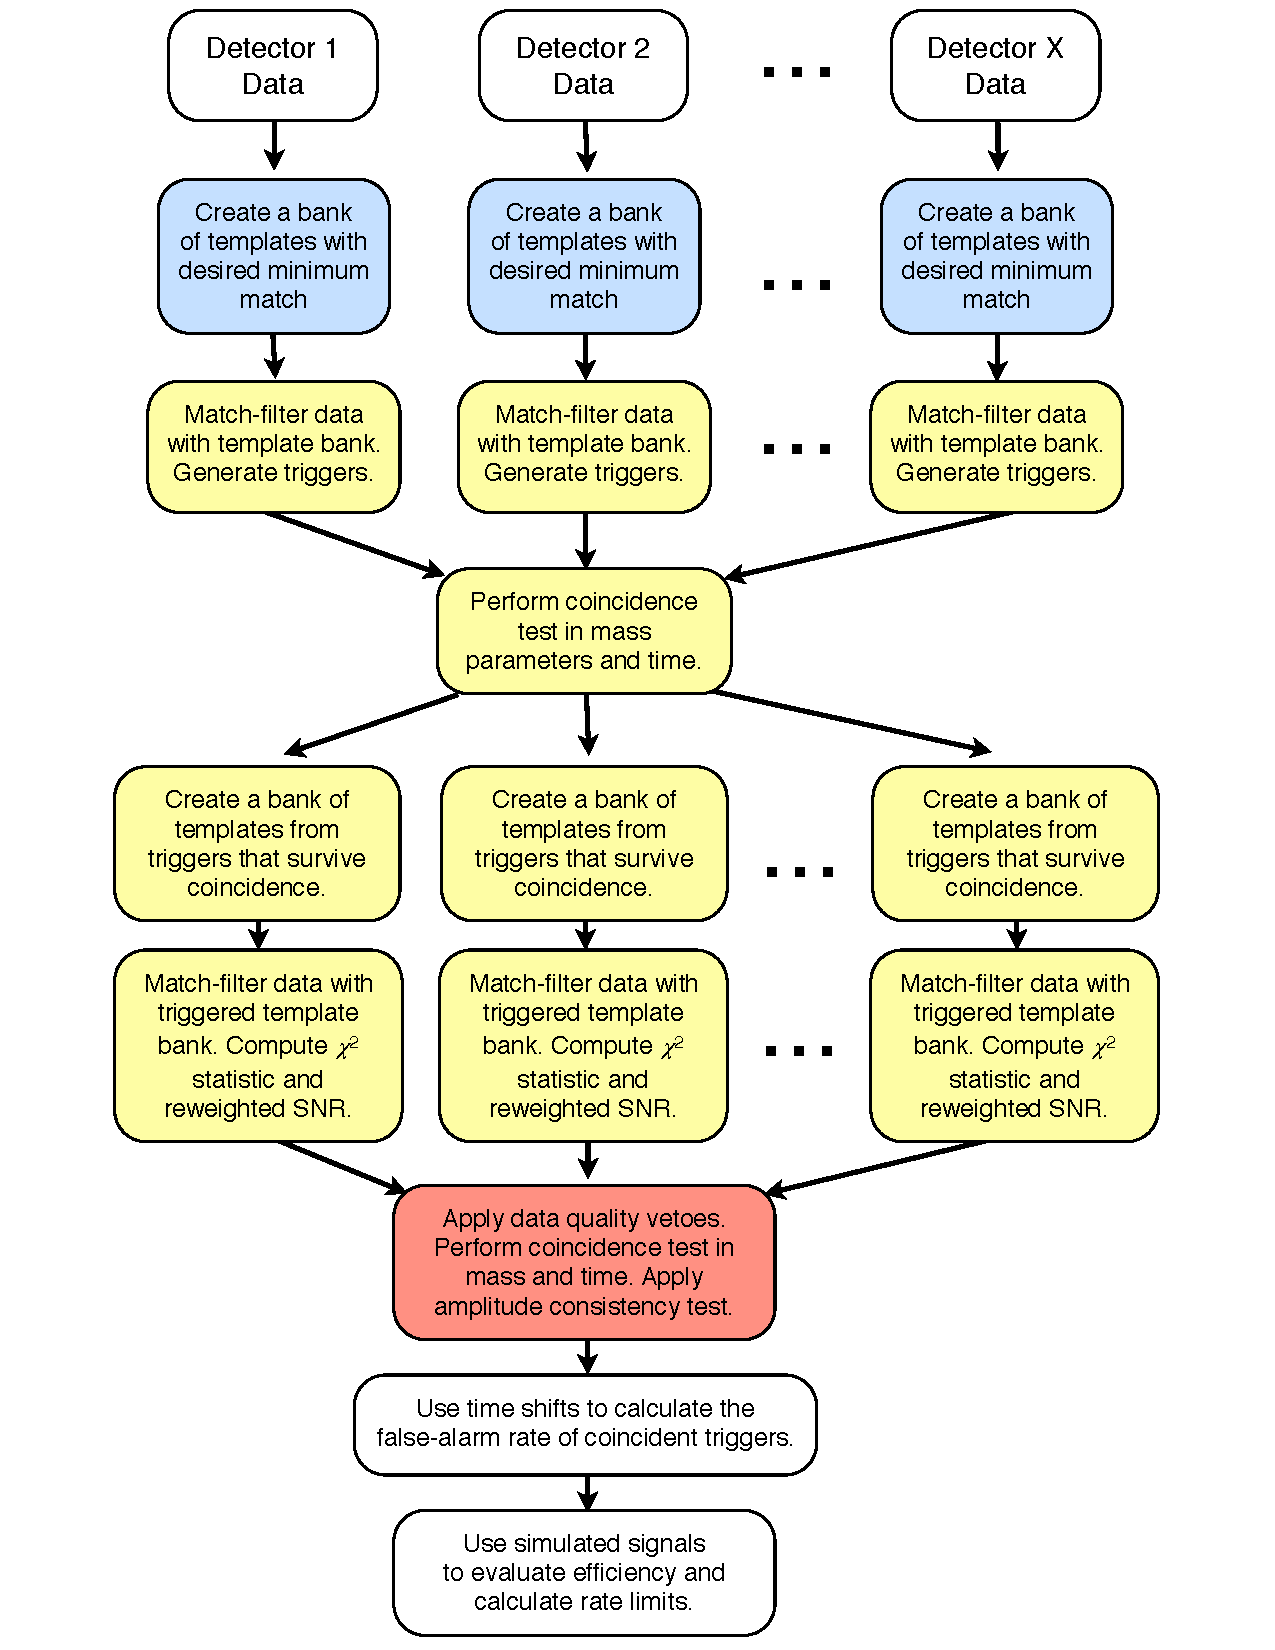
\includegraphics[width=0.47\textwidth,trim=68 22 68 35,clip=true]{figures/two_stage_flowchart.pdf}
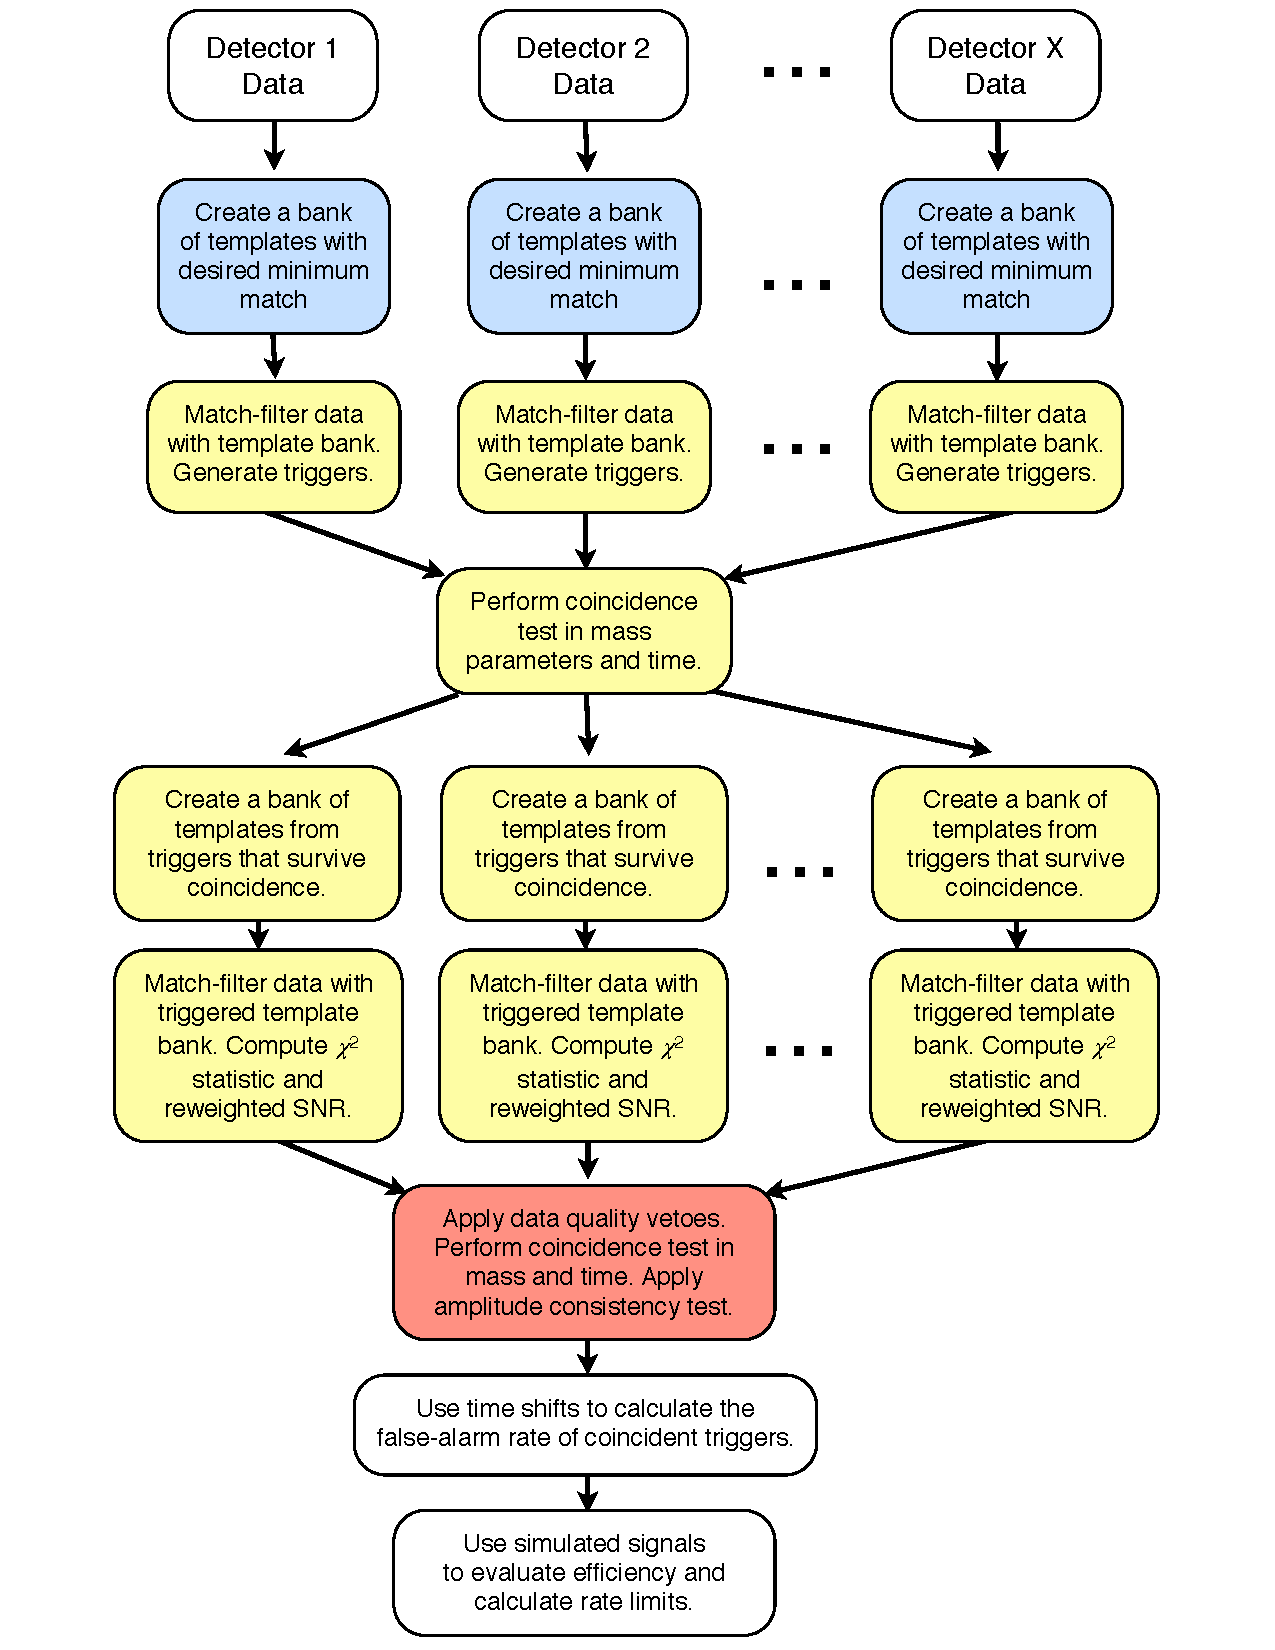
\includegraphics[width=0.47\textwidth,trim=68 22 68 15,clip=false]{figures/two_stage_flowchart.pdf}
\hfill
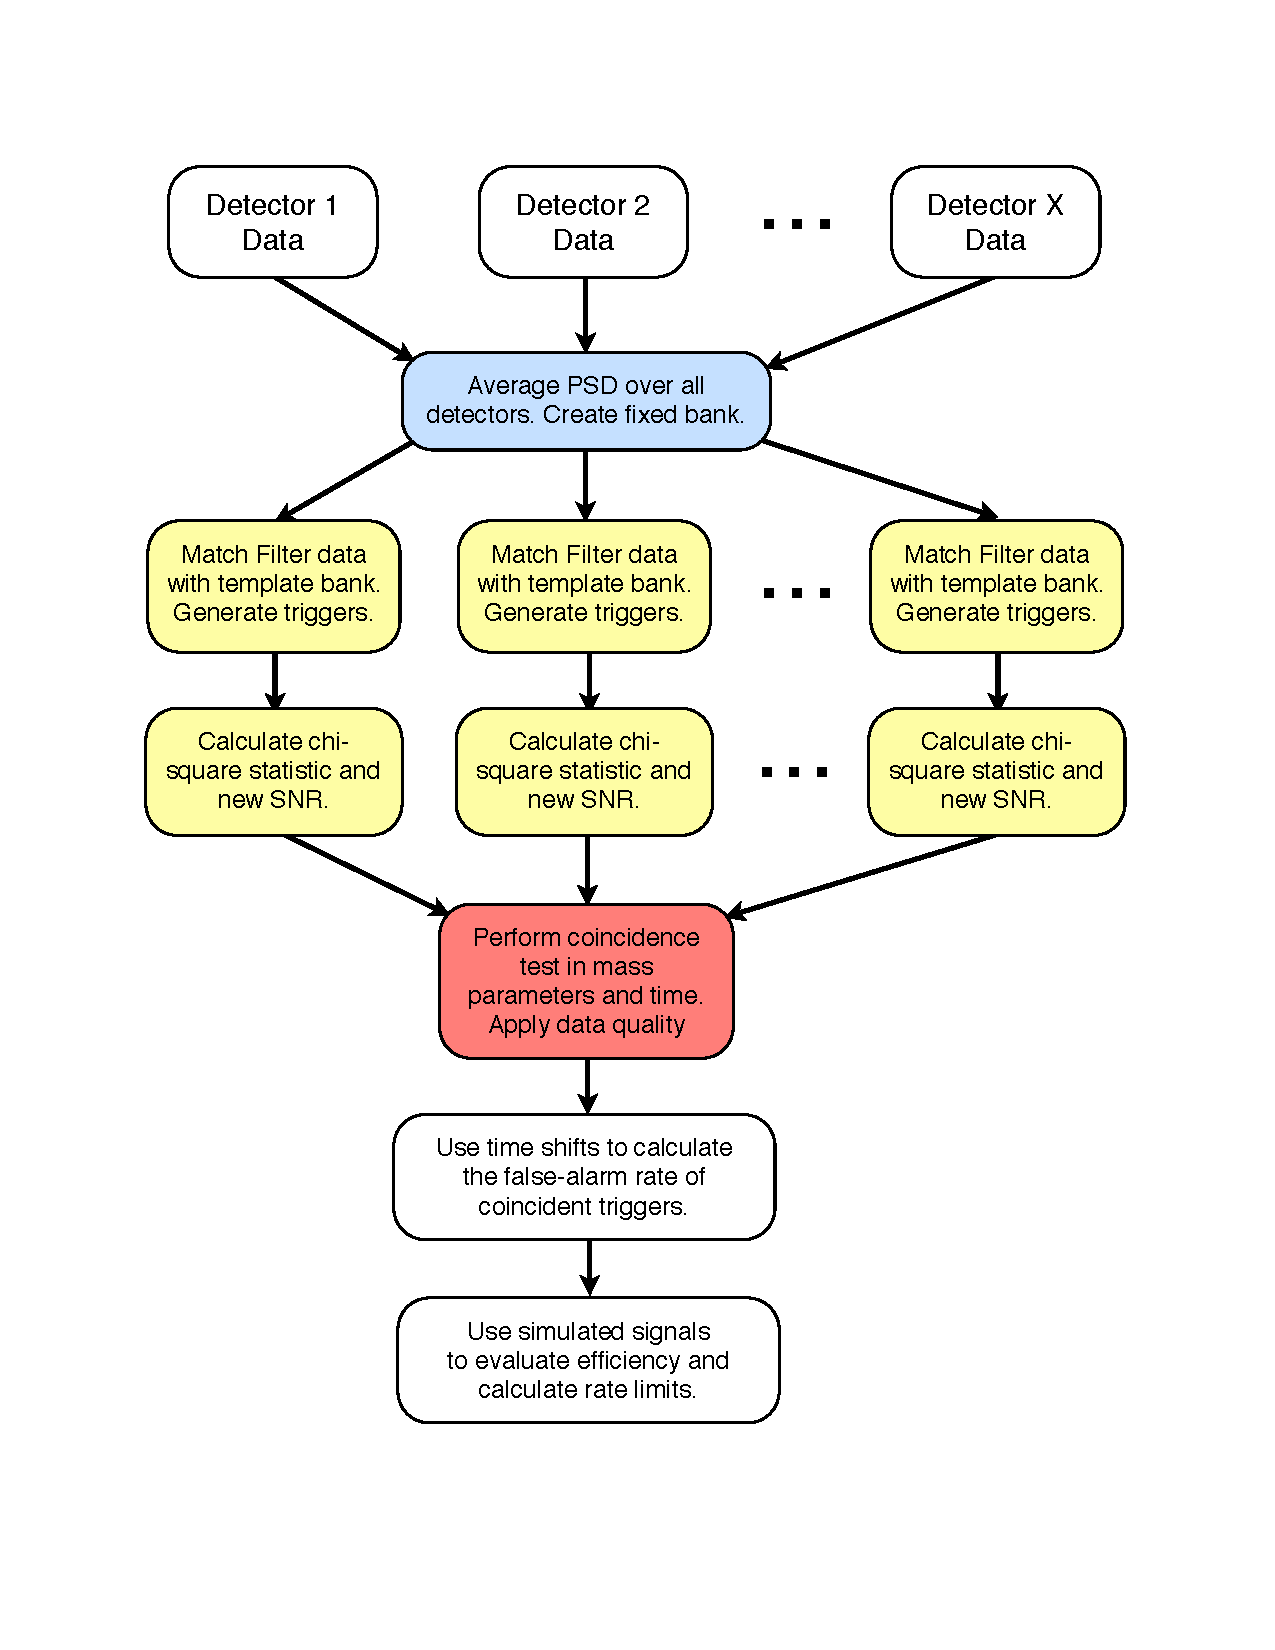
\includegraphics[width=0.47\textwidth,trim=68 -20 68 76,clip=true]{figures/single_stage_flowchart.pdf}
\end{center}
\caption{These flowcharts describe the topologies for the pipeline used in the
S6 search (left) and the final configuration described here (right).  Each
color represents a distinct modification made to the pipeline described in the
different sections in the paper. The yellow is described in
section~\ref{s:stages}, the blue in section~\ref{s:fixed} and the red in
section~\ref{s:coinc}.
\label{fig:pipelines}}
\end{figure}


We first change the workflow of the pipeline from a two-stage pipeline to a
single-stage pipeline, shown by the yellow section of Fig.~\ref{fig:pipelines} 
and described in Sec.~\ref{s:stages}. In the \texttt{ihope} pipeline, a coincidence stage
was applied after computing the matched filter signal-to-noise ratio, but
before computing the $\chi^2$ statistic. The two-stage pipeline was created in
order to avoid performing the computationally expensive $\chi^2$ test on
gravitational-wave candidates that were caused by noise and would be removed
by the computationally cheaper time coincidence test.  However, this lead to
difficulty when estimating the significance of loud gravitational-wave
candidates: only candidates surviving the second round of coincidence testing
had the $\chi^2$ test performed and thus the reweighted signal-to-noise ratio
detection statistic calculated. The single-stage pipeline computes $\chi^2$ 
before coincidence, so that the reweighted signal-to-noise ratio is 
available for all single-detector triggers, allowing the pipeline to estimate 
the false-alarm rate of loud candidates.

We then propose two changes to the placement of the
template bank, shown by the blue section of Fig.~\ref{fig:pipelines}. We
change the bank construction from using a metric accurate to 1.5
post-Newtonian order~\cite{Owen:1998dk} and the placement technique of
Ref.~\cite{Babak:2006ty} to using a metric accurate to 3.5 post-Newtonian
order~\cite{Keppel:2013kia} (the same order as the template waveforms) and the
placement methods described in Ref.~\cite{Brown:2012qf}. We also investigate
several different methods of generating the average power spectral density
of the detectors used to construct the placement metric, including fixing the
power spectral density for bank construction for a week of data, and
averaging the noise spectrum between the two LIGO detectors, so that a shared
bank is used in all detectors.  Finally, in Sec.~\ref{s:coinc}, we investigate a
new type of coincidence test, shown by the red boxes in
Fig~\ref{fig:pipelines}. This test uses the method of
Ref.~\cite{Robinson:2008un} to determine if the triggers are consistent in
time, but requires that the mass parameters of the signal are exactly the same
in the detectors. This test naturally requires using a shared template bank
between detectors, which we construct using the best proposed power spectral
density averaging method.

We test these improvements using two metrics for the performance of the search
pipeline: (i) the ability of the different search pipelines to detect a
distribution of simulated signals injected into the data, called
\emph{software injections}, and (ii) comparing the distribution of coincident
triggers from real LIGO data to that of Gaussian noise. The next
section describes how these tests are performed.

\section{Testing Improvements to the Search}
\label{s:methods}

To test the proposed pipeline improvements, we use data from the S6 LIGO science
run~\cite{Abadie:2011nz}.  Since it is planned that the first aLIGO offline
search will analyze one-week intervals of data, we test the
search pipeline on one-week time intervals. To obtain two representative
times, we examined the sensitivity of the detector, as measured by the
detector's range to a binary neutron star system which would produce a
signal-to-noise ratio of 8 in a single detector.  The BNS inspiral horizon 
distance, shown in Fig.~\ref{img:inspiral-horizon}, is calculated from the
detector's power spectral density~\cite{Abadie:2011nz}.  Therefore, a 
variation in the power spectral density leads to a change in the inspiral 
horizon distance.  For our analysis, we chose the time interval, July 08 to 
July 15, 2010 (blue rectangle in Fig.~\ref{img:inspiral-horizon}), as a week 
when the sensitivity of the detectors changed considerably.  We also 
investigate a second time interval of L1 and H1 data, the week from August 
14-21, 2010 (black rectangle in Fig.~\ref{img:inspiral-horizon}) with a more
stable range to verify our results.
We also re-analyzed these two weeks replacing the LIGO data with simulated
stationary Gaussian noise, colored with the design spectrum of the initial LIGO detectors.
To compare the performance of the pipeline in real data to its performance in
Gaussian noise, we show histograms of the combined reweighted signal-to-noise ratio for coincidence
background candidates  obtained from analyzing Gaussian noise and from
analyzing LIGO data. These histograms allow us to determine the search
pipelines' ability to eliminate non-Gaussian noise transients in the LIGO
data.

\begin{figure}[tbp]
\begin{center}
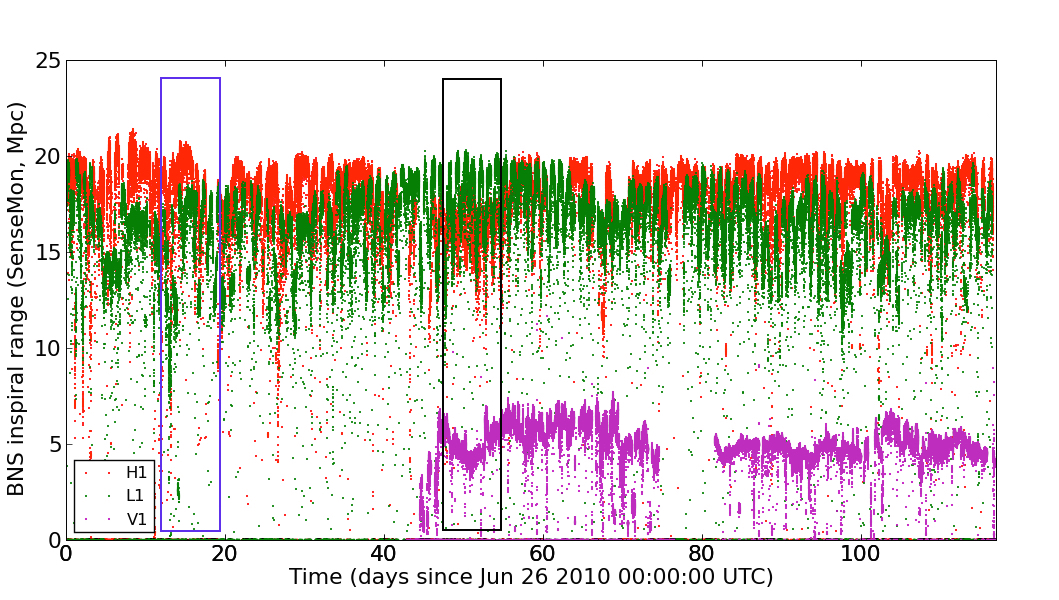
\includegraphics[height=8cm]{figures/s6d-inspiral_range-intervall.png}  % preprint size
\caption{Sensitivity of the gravitational-wave detectors 
for the last part of the sixth science run for LIGO (S6D) and the third VIRGO science run (VSR3). 
The plot shows the volume-weighted average distance at which a 1.4, 1.4 BNS would be
observed with an signal-to-noise ratio of 8 for each detector. %Cite? 
The two rectangles indicate time intervals used for this study. 
%The BNS inspiral horizon distance of a detector is given by the distance at which an optimally oriented 
%binary system of two compact objects with $1.4 \ \text{M}_{\odot}$ would create a SNR of 8~\cite{LIGO:2012aa}.
%The SenseMon range shown on the left axis is obtained by dividing the inspiral 
%horizon distance by 2.26. This corresponds to the average over all sky locations 
%and positions of the system \cite{LIGO:2012aa}. 
%The inspiral horizon distance for the whole sixth science run for LIGO can be found in 
%\cite{capano2012searching}.
}
\label{img:inspiral-horizon}
\end{center}
\end{figure}

As the primary metric of search sensitivity, we measure the sensitivity of a 
pipeline by finding the \emph{sensitive
volume}, which is proportional to the number of detections a pipeline will
make per unit time at a given false-alarm rate. This is given by:
\begin{equation}
V(F) = \int \epsilon(F; r, \Omega, \mathbf{\Lambda}) p(r, \Omega, \mathbf{\Lambda}) r^2 \mathrm{d}r \mathrm{d}\Omega \mathrm{d}\mathbf{\Lambda}.
\end{equation}
Here, $\mathbf{\Lambda}$ are the physical parameters of a signal (in this
study, $\{m_1, m_2\}$), $p(r, \Omega, \mathbf{\Lambda})$ is the distribution of
signals in the universe, and $\epsilon$ is the efficiency of the pipeline at
detecting signals at a distance $r$, sky location $\Omega$, and false-alarm
rate $F$.

We estimate the sensitive volume by adding to the data a large number of
simulated signals (\emph{injections}) that are randomly drawn from a
distribution $q(r, \Omega, \mathbf{\Lambda})$. 
We assume an isotropic random distribution of sky positions and orientations.
Masses are distributed uniformly in component mass, with the bounds dependent
on the type of compact object: $m \in [1,3]\,\mathrm{M}_\odot$ for neutron
stars (NS); $m \in [1,13]\,\mathrm{M}_\odot$ for black holes (BH). We also
restrict the total masses of binaries to be $\leq 14\,\mathrm{M}_\odot$. We
allow template banks to extend to a total mass of $25\,\mathrm{M}_\odot$,
as shown in Fig~\ref{Inj-massrange}. We assume approximately equal rates of
BNS, NSBH, and BBH systems. Injections are generated at 3.5 PN order in the
time domain using the TaylorT4 approximant.

We re-analyze the data with these simulated signals added and,
for each injection, determine if a coincident trigger is present within 1
second of the time of the injection. If a trigger is present, we use the
combined reweighted signal-to-noise ratio to compute its false-alarm rate. 
If no trigger is present, the injection is
\emph{missed}, i.e., the signal cannot be distinguished from noise at any
false-alarm rate
threshold. At some distance $r_{\max}$ we expect that any signal with $r >
r_{\max}$ will be missed.  Likewise, within some distance $r_{\min}$ we expect
that nearly every signal will be
found, even at an extremely small ($\lesssim 10^{-4} / \mathrm{yr}$)
false-alarm rate
threshold. These bounds depend on the physical parameters of a signal.
Gravitational waves from more massive systems have larger amplitudes, and thus
can be detected at greater distances than less massive systems. To first order,
if a binary with a reference \emph{chirp mass} $\mathcal{M}_0 = (m_1
m_2)^{3/5}/(m_1 + m_2)^{1/5}$ is detected at a distance $r_0$, then a binary
with arbitrary chirp mass $\mathcal{M}$ will be detected with approximately the
same reweighted signal-to-noise ratio at a distance:
\begin{equation}
r = r_{0}(\mathcal{M}/\mathcal{M}_{0})^{5/6}.
\label{eqn:chirp_distance}
\end{equation}
We find that $r_{\min} = 0.5\,$Mpc and $r_{\max} = 30\,$Mpc are reasonable
bounds for a binary in which both component masses are $1.4\,\mathrm{M}_\odot$.
For each injection, we scale these bounds using Eq. \eqref{eqn:chirp_distance},
then draw the distance uniformly between them. The sensitive volume
is then simply an average over the total number of injections $N$:
\begin{equation}
V(F) \approx \frac{1}{N} \sum_{i=1}^N g_i(F) \equiv \left<g(F)\right>,
\end{equation}
where:
\begin{equation}
g_i(F) = \frac{4\pi}{3} \left[ r_{\min,i}^3 + 3r_i^2(r_{\max,i}-r_{\min,i})\hat{\epsilon}(F; F_i, r_i, \Omega_i, \mathbf{\Lambda}_i)\right].
\end{equation}
Here, $\hat{\epsilon} = 1$ if $F_i \leq F$, and
$0$ otherwise. The error in the estimate is:% \cite{ref:num_methods}:
\begin{equation}
\delta V = \sqrt{\frac{\left<g^2\right> - \left<g\right>^2}{N}}.
\end{equation}

\begin{figure}[tbh]
\begin{center}
	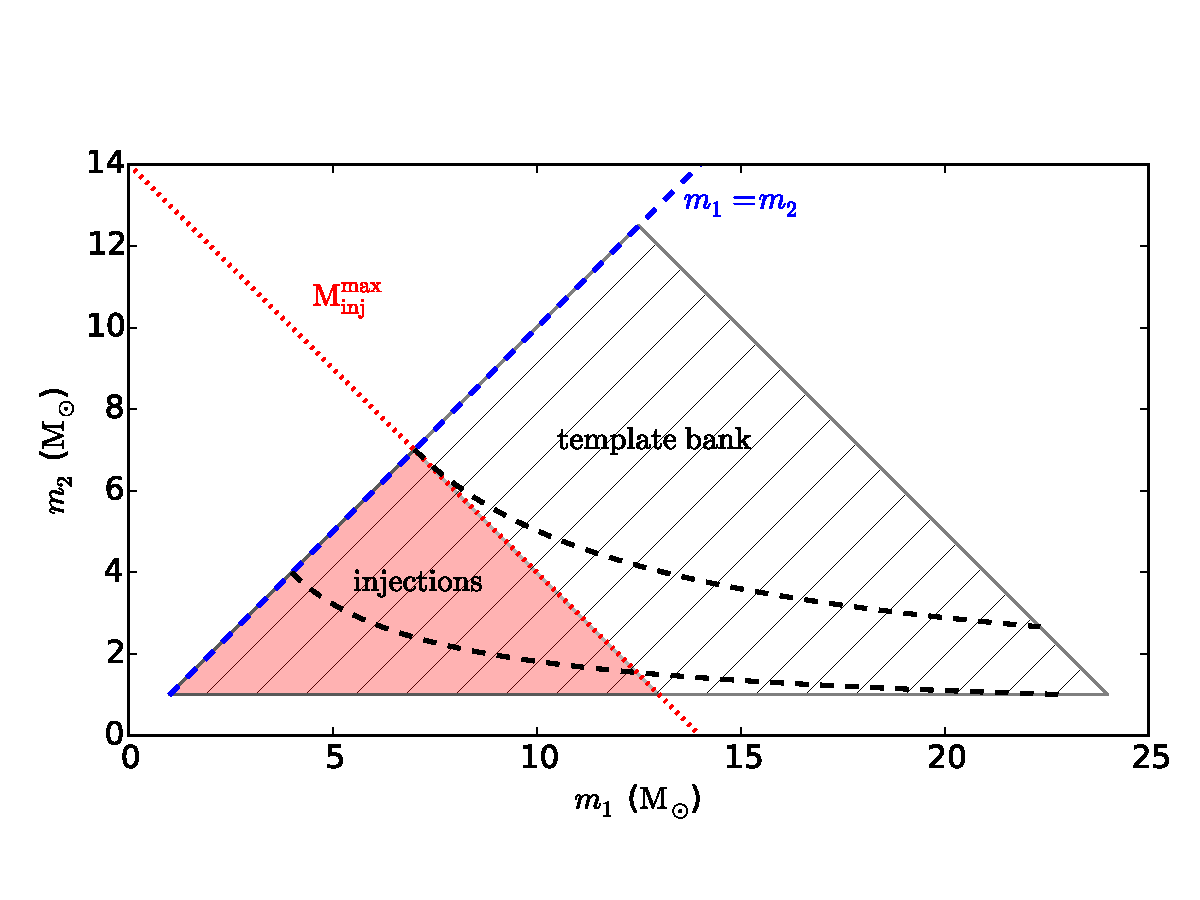
\includegraphics[width=0.7\textwidth]{figures/lowmass-inj.pdf} 
\caption{Mass-ranges for software injection, shown in the $m_1-m_2$
mass-plane.  As customary, we restrict to $m_1\ge m_2$. The template bank
used to search for these injections is indicated by hatched regions and the
injection set by the red shaded region. The black dashed line shows a chirp
mass of $3.48\ M_\odot$, the boundary between the two mass bins used. Triggers
from templates with chirp masses larger than $6.1\ M_\odot$ are discarded in
post-processing.
}
\label{Inj-massrange}
\end{center}
\end{figure}

\section{Search Sensitive Volume Comparison}
\label{s:results}

We have performed a total of eight different analyses to test our proposed
changes. These are summarized in Table~\ref{table:search}.  The first analysis
used the two-stage \texttt{ihope} search pipeline in the same configuration
originally used in the S6/VSR2,3 search for low-mass compact binaries. Each
successive analysis represents a single modification from the previous search.
Thus, the effect each change has on the search pipeline's sensitivity can be
individually noted. For each analysis, we compute the sensitive volume as a
function of false-alarm rate, and for analyses 1, 2, and 7 we also compare the
distribution of background triggers in LIGO data to that of Gaussian noise.

\begin{table}[tbh]
\begin{center}
{\small
\begin{tabular}{|c|c|c|c|c|c|c|}
\hline 									
Analysis & Pipeline & Bank & Bank PSD   & Detector & Bank PSD	& Coincidence	\\
         &          & Metric & estimation & banks  & Averaging & \\
\hline 							
\hline 																
1 & \splitcell{Two-stage \\ \texttt{ihope}} & \multirow{3}{12mm}{1.5 pN} & \multirow{5}{20mm}{\splitcell{Regenerated\\ every \\ 2048 s}} & \multirow{5}{14mm}{Separate} & \multirow{4}{14mm}{N/A} & \multirow{7}{14mm}{Ellipsoid}  \\ \cline{1-2}
2 & \splitcell{Single-stage \\ \texttt{ihope}} & & & &	         	&	\\ \cline{1-1} \cline{2-2}
3 & \multirow{6}{20mm}{\splitcell{Single-stage \\ \texttt{PyCBC}}} & & & &	         	&	\\ \cline{1-1} \cline{3-3}
4 & & \multirow{5}{12mm}{3.5 pN} & & & & \\ \cline{1-1 }\cline{6-6}
5 & & & & & 	\multirow{2}{14mm}{Harmonic}	&       \\ \cline{1-1} \cline{4-5}	
6 & & & \multirow{3}{14mm}{\splitcell{Fixed\\ for \\ week}} & \multirow{3}{14mm}{Shared} & &       \\ \cline{1-1} \cline{6-6}
7 & & & & & Smallest-Value	&       \\ \cline{1-1} \cline{6-7}				
8 & & & & & Harmonic	&	Exact-match	\\ \hline
\end{tabular}		
}
\end{center}
\caption{Overview of the eight different analysis performed to test
improvements to the search pipeline in this paper. Each successive analysis
incorporates a change from the previous search pipeline. The pipeline column
indicates the pipeline workflow and the software used to run the search. The
bank metric column indicates whether templates are placed using a metric
accurate to 1.5 pN or 3.5 pN order. The bank power spectral density (PSD) 
estimation column indicates whether the template bank was placed using a power 
spectral density re-computed every 2048
seconds, or if the search used one fixed template bank for the entire week.
The detector banks column indicates whether a seperate template bank was 
generated for each detector, or if the template bank was shared by both
detectors. For fixed template banks, the bank power spectral density averaging column gives the
type of power spectral density averaging used over the week to generate place the bank. The
coincidence column indicates whether the analysis used the ellipsoidal
coincidence method or the exact-match coincidence method.
\label{table:search}
}
\end{table}


\subsection{Single-Stage Pipeline Workflow}
\label{s:stages}

Our analysis begins with pipeline used in LIGO's sixth science run. This
pipeline, shown on the left in Fig.~\ref{fig:pipelines}, was a two-stage
pipeline, so called because there are two times that the coincidence test is
applied.  The two-stage process was created in order to avoid performing the
computationally expensive $\chi^2$ test on gravitational wave candidates that
were caused by noise and would be removed by the computationally cheaper time
coincidence test. For this reason, the coincidence test was performed before
the $\chi^2$ test. 

The two-stage \texttt{ihope} pipeline was very effective at downweighting the 
significance of triggers due to noise.  Fig.~\ref{fig:2s_bg} shows two histograms
of gravitational-wave candidates as a function of reweighted signal-to-noise ratio that survived
time-lagged coincidence tests. The red lines in the figure are from an
analysis of Gaussian noise, while the black lines denote an analysis of real
LIGO data. The plots demonstrate that the two-stage pipeline downweights
significant noise-generated triggers to the point that the LIGO data is very
close to the analysis of Gaussian noise.

However, the two-stage workflow led to difficulty when estimating the
significance of surviving gravitational-wave candidates: only candidates
surviving the second round of coincidence testing had the $\chi^2$ test
performed and thus the new detection statistic calculated.  In the
S6/VSR2,3 search the pipeline used 100 time shifts, each with a 5 second 
offset, limiting the significance that can be measured.  For 
loud gravitational-wave candidates, further background estimation must be
performed to calculate false-alarm rates at less than one in a thousand years.
To calculate this extended background, the data is offset by multiples of $0.2$ seconds to
perform a coincdence test. This is done as many times as possible, and the
resulting coincident triggers are used to estimate a false-alarm rate. 
computing as many time shifts as possible, while coincident data remains.

In the S6/VSR2,3 analysis, applying this extended background estimation 
required re-analysis of the data with the $\chi^2$ test turned on at the 
first stage, eliminating any computational savings 
of the two-stage pipeline. Furthermore, although the output of the two-stage
pipeline should be identical to a single-stage pipeline, in practice the
two-stage pipeline does not produce the same triggers. This is primarily due
to the fact that the single-detector triggers are clustered in a 30~ms window
over the template bank after the first matched-filtering jobs, and then fed
back into the search as a new bank after coincidence~\cite{Babak:2012zx}. This
non-linearity adds additional complication when testing and tuning the
pipeline.


For both of these reasons, although primarily for the false alarm-rate
considerations, it is desirable to abandon the two-stage pipeline and switch
to a simpler single-stage workflow, as shown on the right in
Fig.~\ref{fig:pipelines}.  The single-stage pipeline essentially rearranges
the previous pipeline computing the $\chi^2$ test before the coincidence test
and removing the triggered template bank generation and the second
match-filter process.  Fig.~\ref{fig:ss_bg} shows the background triggers
as a function of reweighted signal-to-noise ratio of the single-stage analysis 
of S6 data compared to a
those of a single-stage analysis of Gaussian data. Like the two-stage
pipeline's performance shown in Fig.~\ref{fig:2s_bg}, we see the
single-stage pipeline is also successful in removing candidates with high
significance.  The single-stage pipeline is expected to perform identically to
the two-stage pipeline. Fig.~\ref{fig:roc1} compares the sensitive volumes
of these search pipelines. The sensitive volume measurement for the two-stage
pipeline terminates at a false-alarm rate of order one per year, limited by
the 100 time-slides performed by the two-stage pipeline. However, with
the single-stage pipeline, many more time-slides can be performed and the
false-alarm rate of injections can be computed down to of order $1/10,000$
years using one week of data. We can see that in the region where both can
compute the false-alarm rate of triggers, the sensitivities of the two
pipelines agree as expected.

\begin{figure}[tbp]
\begin{center}
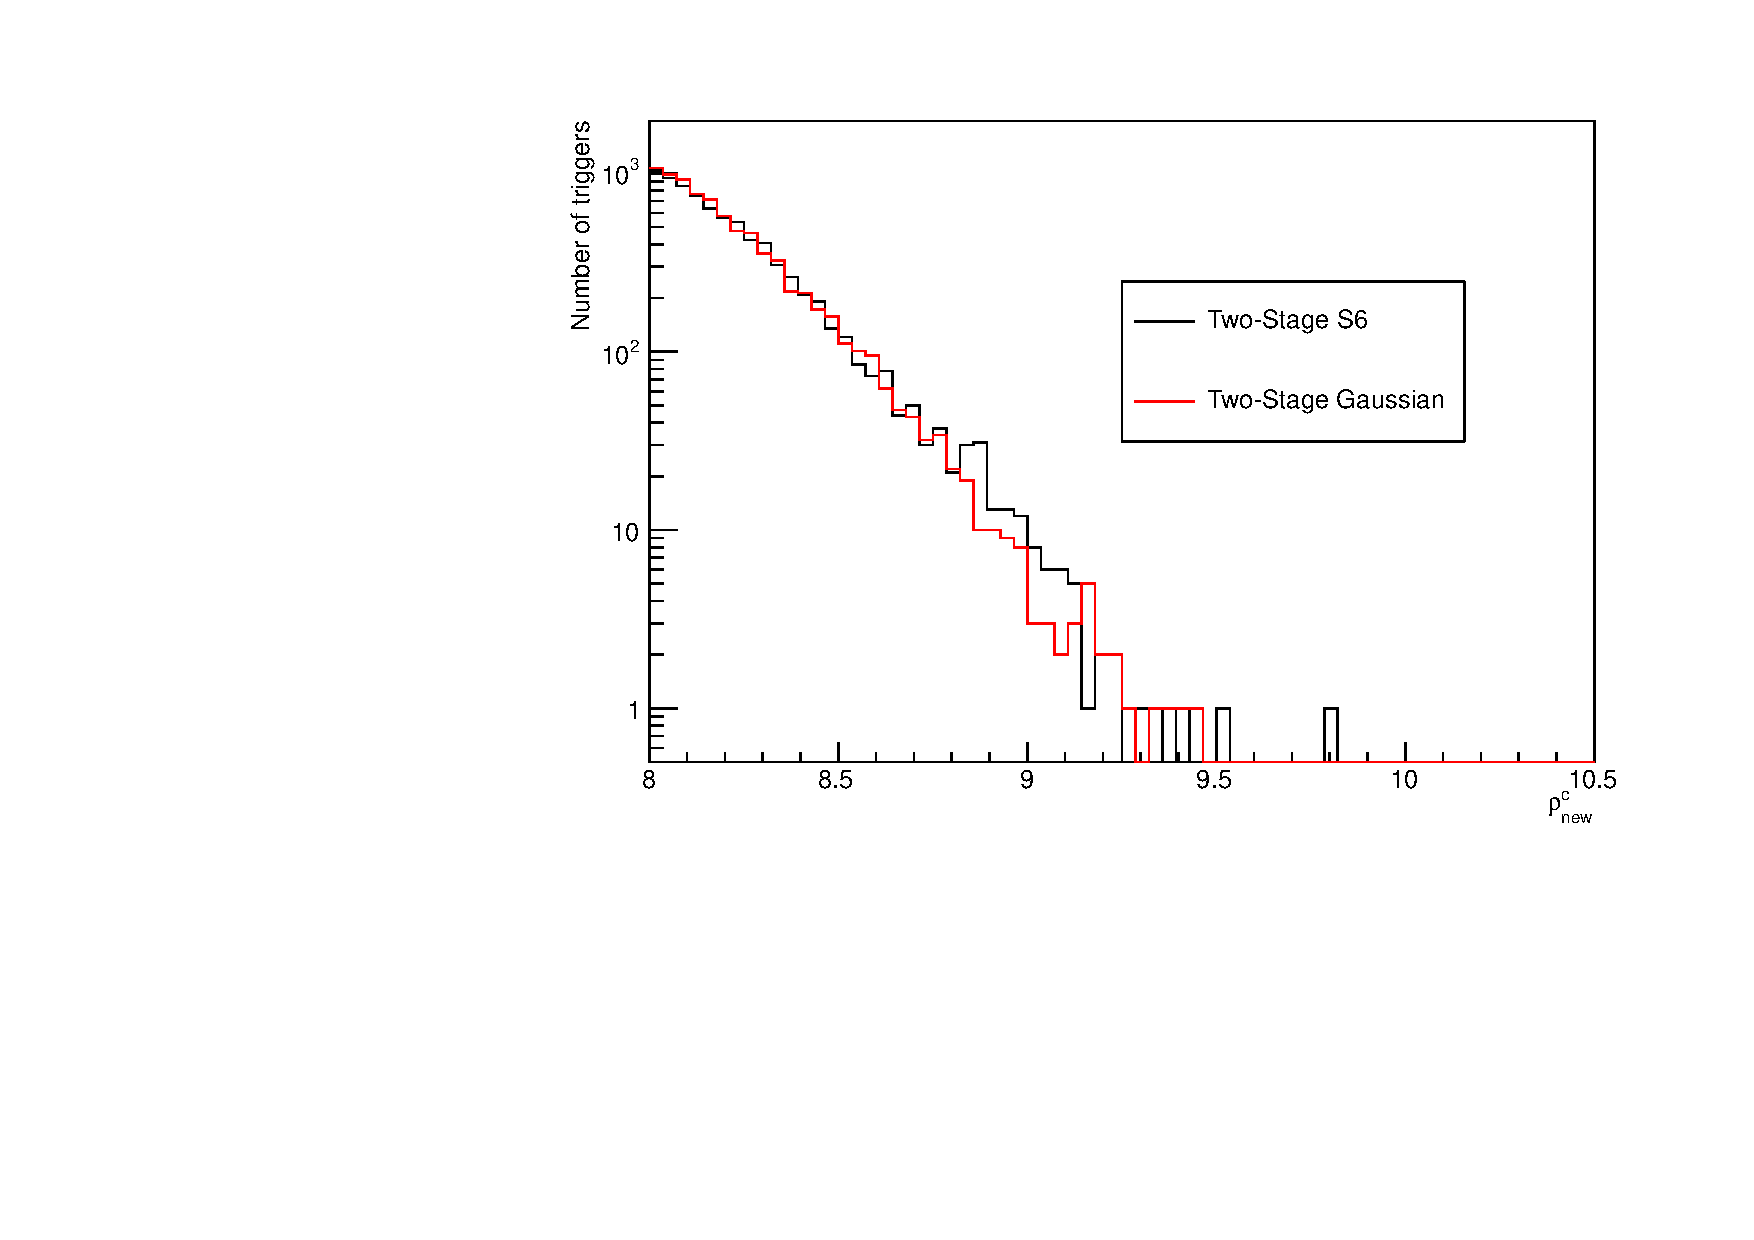
\includegraphics[width=0.45\textwidth]{figures/histograms/two_stage_hist_w1.pdf} 
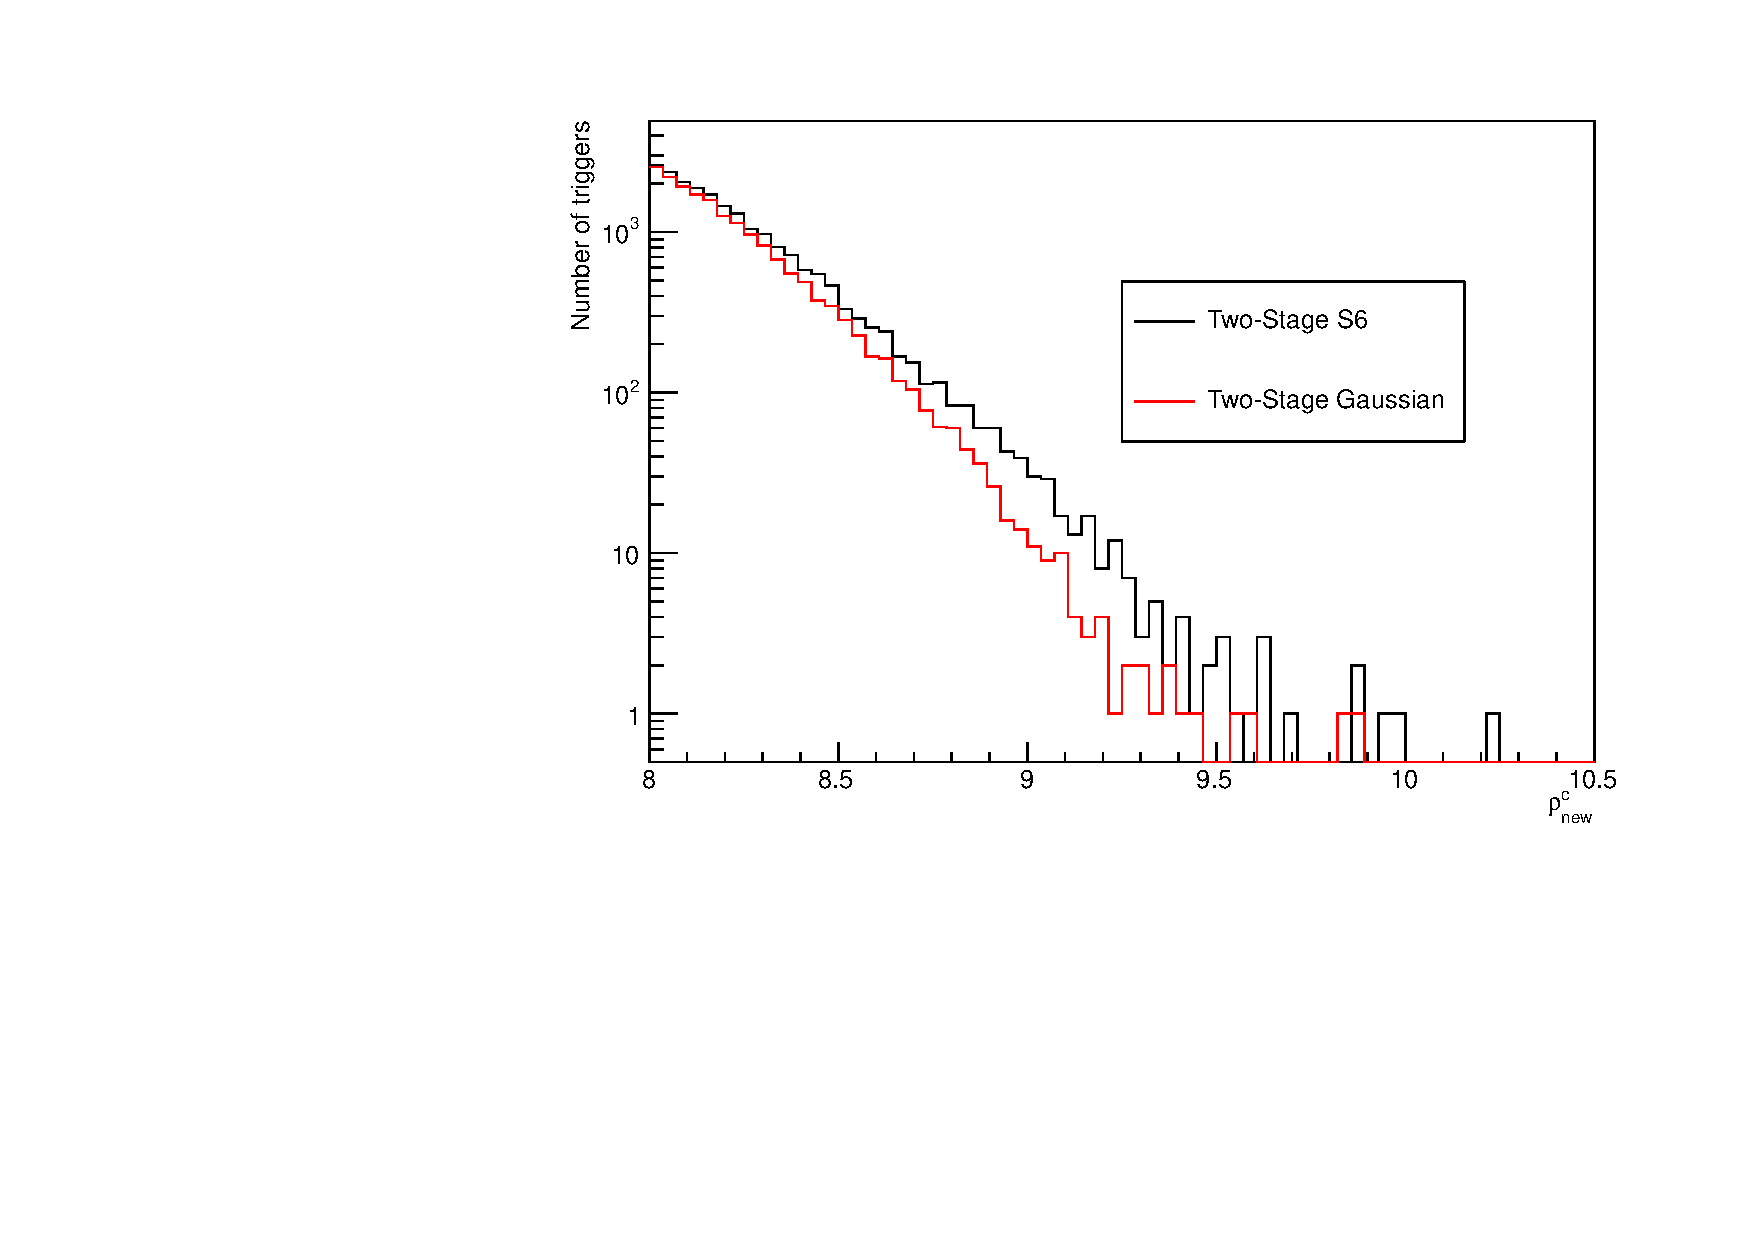
\includegraphics[width=0.45\textwidth]{figures/histograms/two_stage_hist_w2.pdf} 
\caption{This histogram shows the number of background triggers that survived
coincidence testing from the two-stage analyses. They are categorized in bins
of combined reweighted signal-to-noise ratio. The left plot represents an 
analysis of a week of data from
July 2010 while the right plot represents an analysis of a week of data from August 2010. The
red line denotes the background triggers from the Gaussian analysis. The black
line denotes the background triggers from the first S6 data analysis.}
\label{fig:2s_bg}
\end{center}
\end{figure}

\begin{figure}[tbp]
\begin{center}
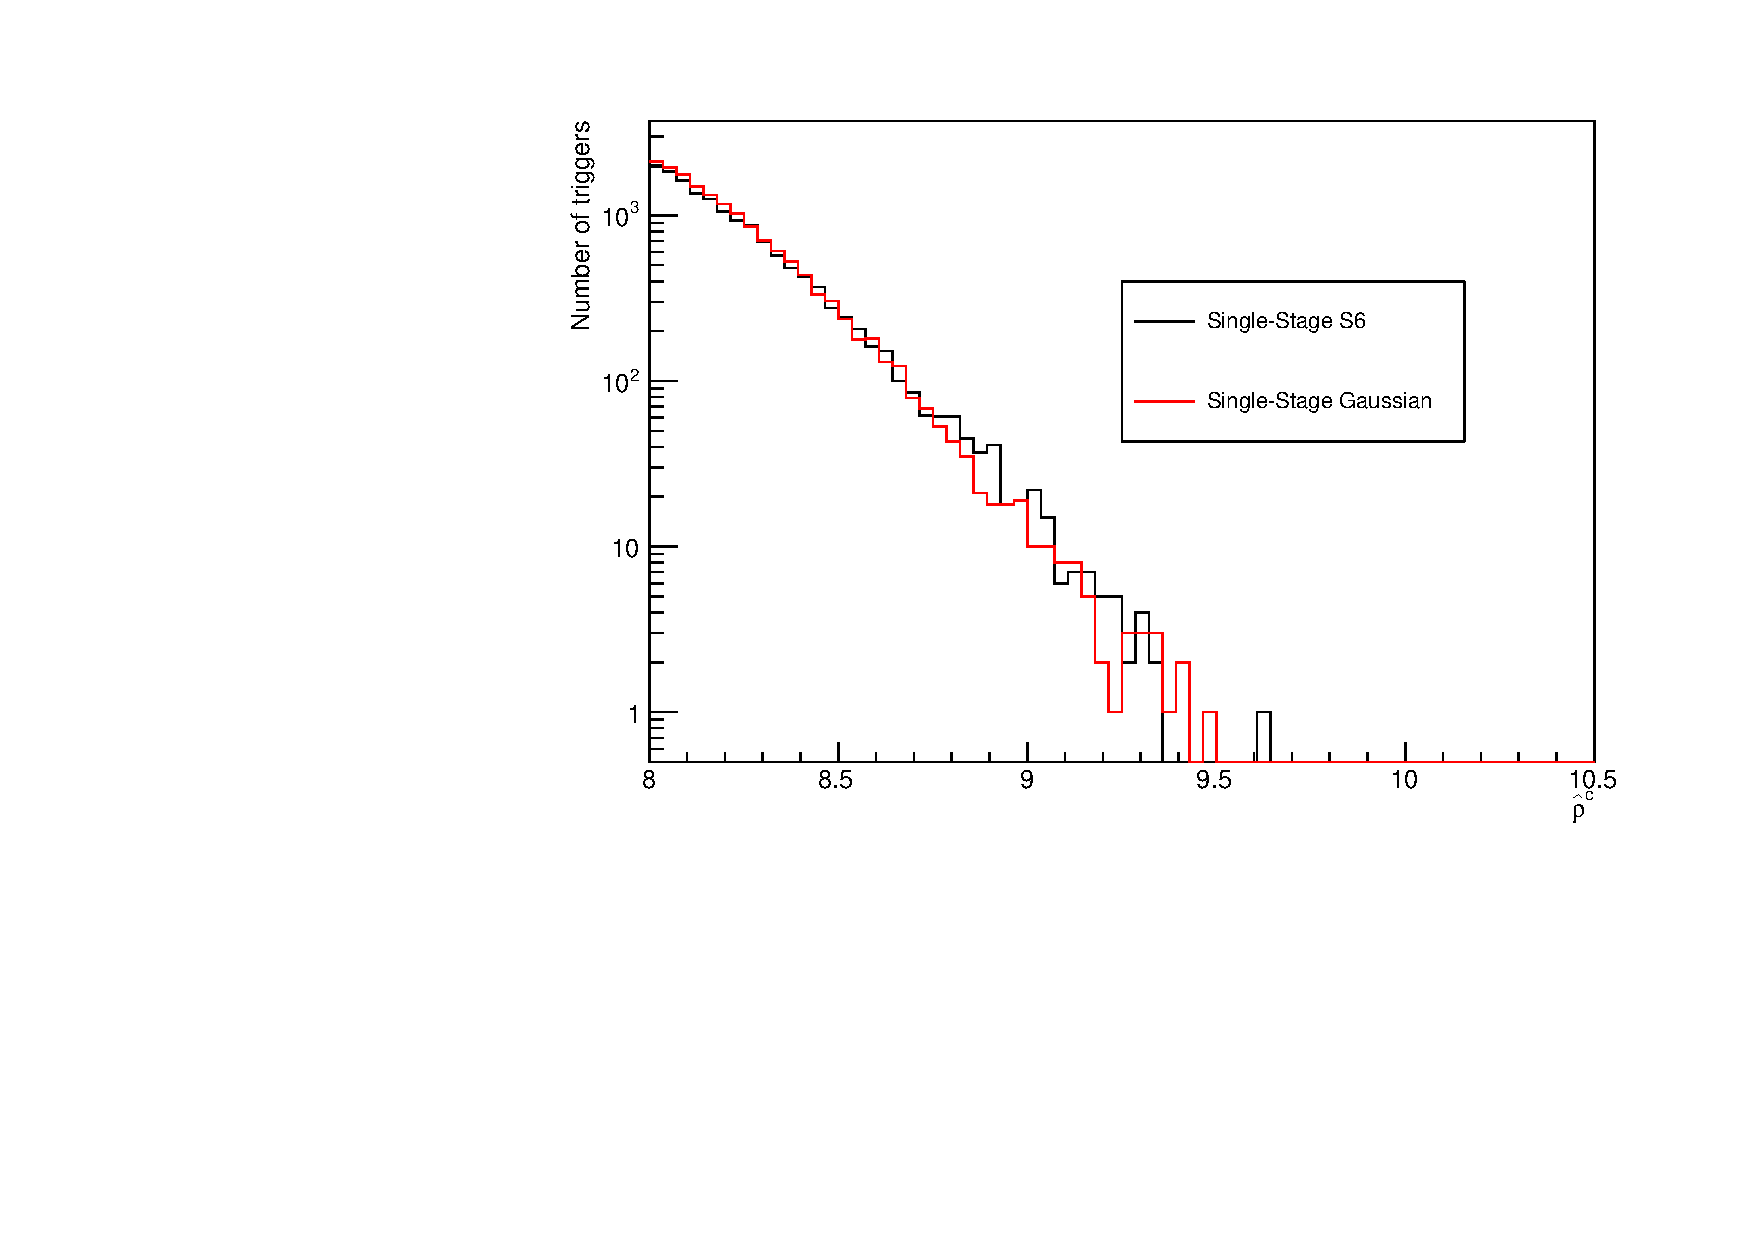
\includegraphics[width=0.45\textwidth]{figures/histograms/single_stage_hist_w1.pdf}
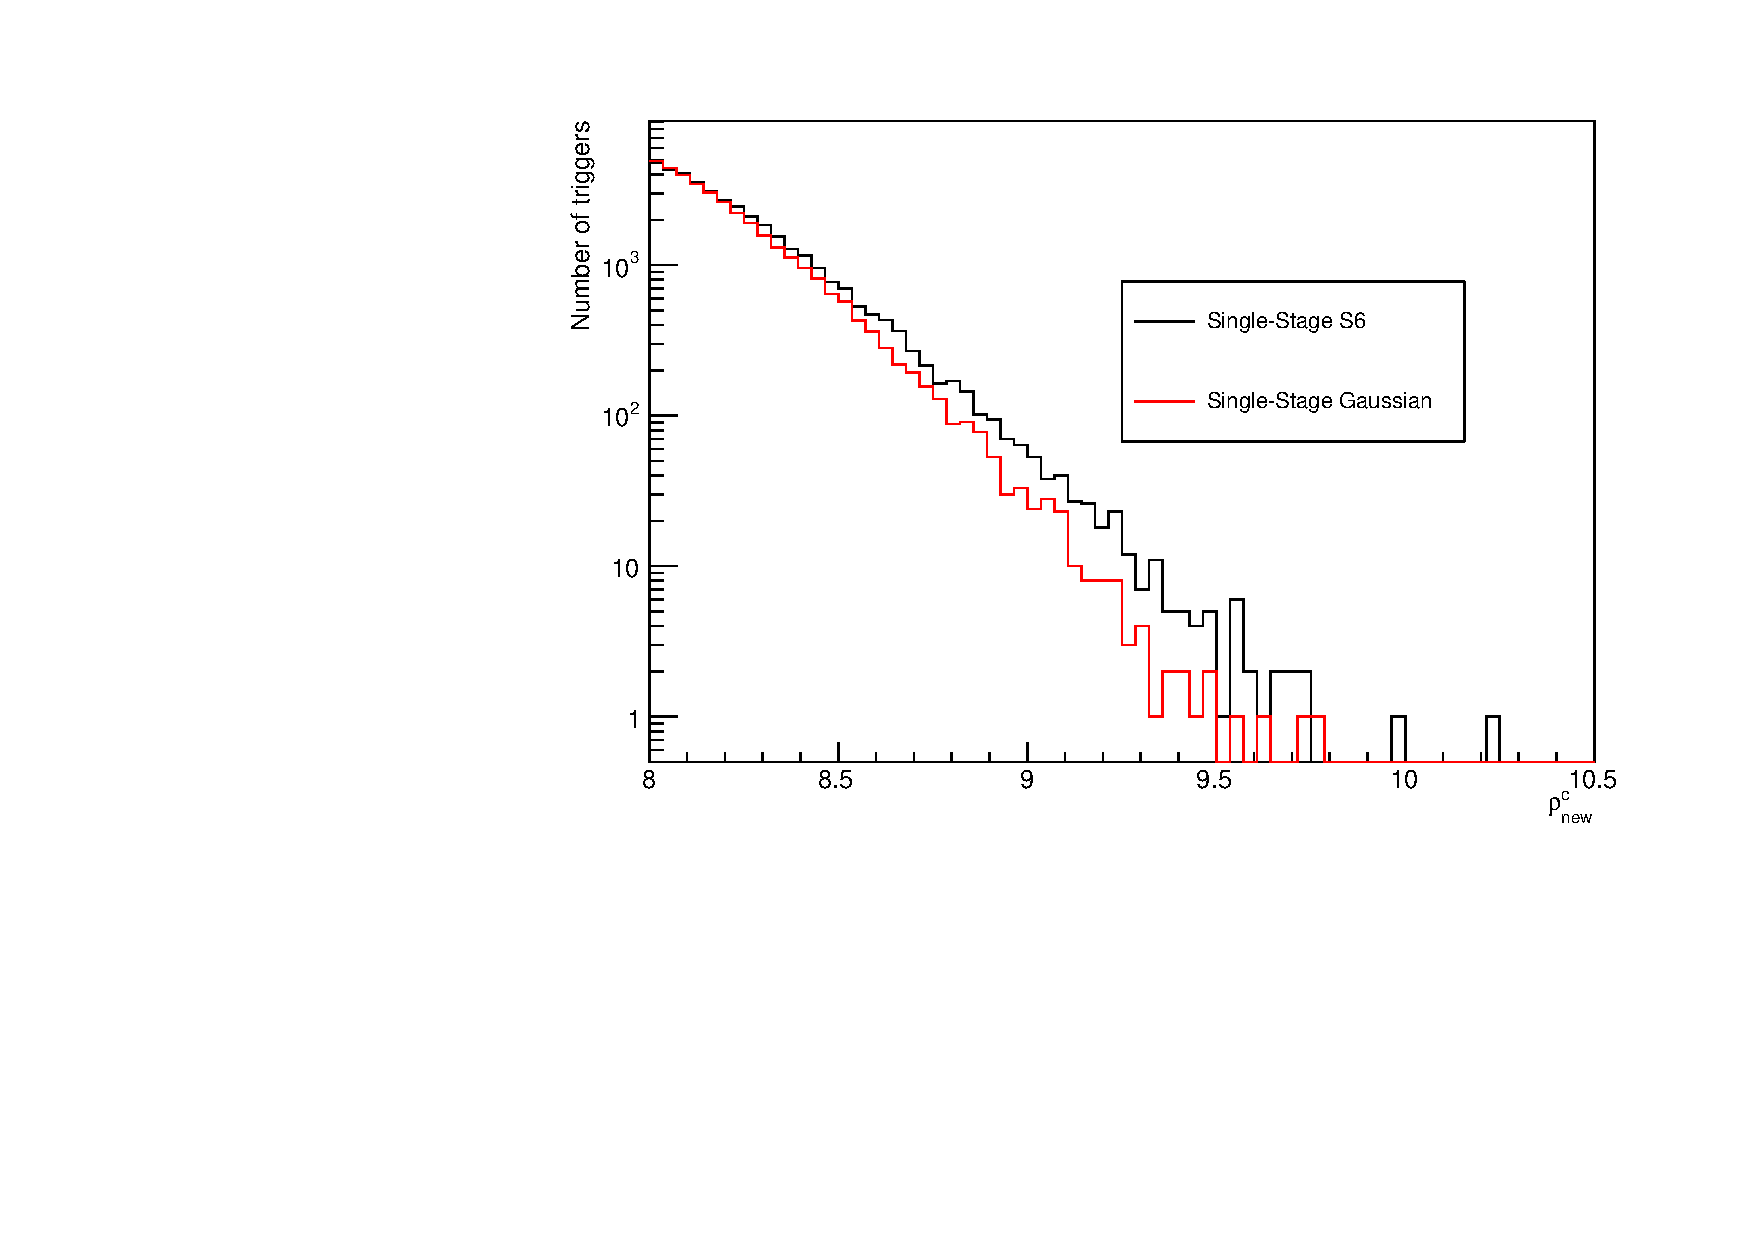
\includegraphics[width=0.45\textwidth]{figures/histograms/single_stage_hist_w2.pdf}
\caption{This histogram shows the number of background triggers that survived
coincidence testing from the single stage analyses in different bins of
combined reweighted signal-to-noise ratio. The left plot represents a week 
analysis of data from July
2010 while the right plot represents an analysis of a week of data from August 2010. The red
line denotes the background triggers from the Gaussian analysis. The black
line denotes the background triggers from the first S6 data analysis.}
\label{fig:ss_bg}
\end{center}
\end{figure}

\begin{figure}[tbp]
\begin{center}
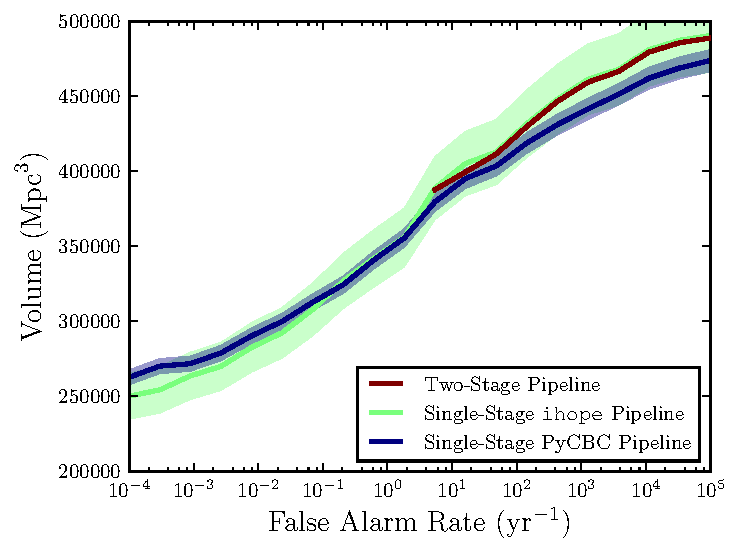
\includegraphics[width=0.45\textwidth]{figures/volume_plots/two_and_single_stage_w1_volume.pdf}
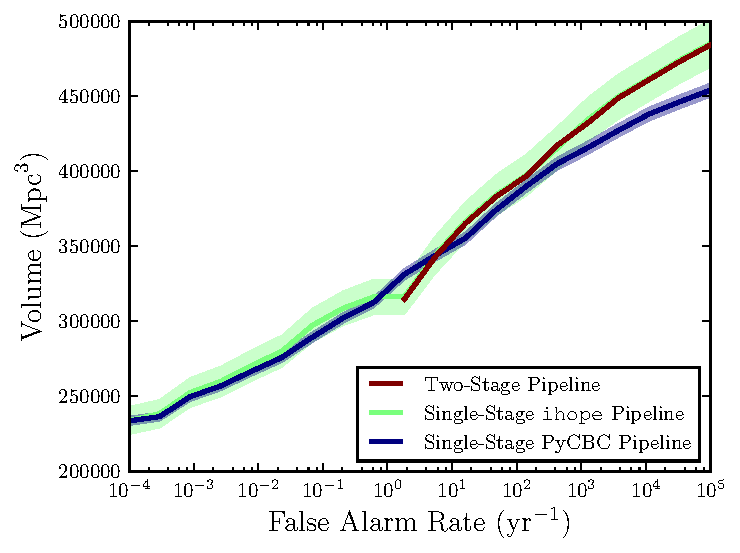
\includegraphics[width=0.45\textwidth]{figures/volume_plots/two_and_single_stage_w2_volume.pdf}
\caption{This plot gives the relative sensitive volume of the two-stage
analysis to the single-stage analysis as a function of the false-alarm rate
In the region above a false-alarm rate of
$\sim 2$ per year, where both pipelines can measure the false-alarm rate of
candidates, the sensitivity of the two pipelines is the same. By performing
many more time shifts to estimate the background, the single-stage pipeline
can estimate the significance of triggers to a false-alarm rate of $\sim
10^{-4}$ per year using one week of data. We also include an analysis with the
same pipeline workflow as the single-stage pipeline, but that uses the new
\texttt{PyCBC} search code, instead of the previously-used \texttt{ihope}
code. The error bars on the \texttt{PyCBC} search are smaller, as the increased
computational efficiency of this pipeline allows us to perform an order of
magnitude more injections. However, the results otherwise agree. The left plot
represents an analysis of a week of data from July 2010 while the right plot represents a week
analysis of data from August 2010.}
\label{fig:roc1}
\end{center}
\end{figure}

As described above, the primary motivation for the two-stage pipeline was to
mitigate the computational cost of the signal-based vetoes.  If triggers are
found above threshold, the $\chi^2$ time-frequency signal consistency test is
applied.  The test consists of breaking the waveform into $p$ frequency bins
of equal power. Each bin is filtered against the data to obtain the partial
signal-to-noise ratio contribution $\rho_l$ and then compared to the expected 
signal-to-noise ratio contribution $\rho/p$. 
In the \texttt{ihope} pipeline, the value of the $\chi^2$ statistic was
computed as a function of time for a template if there were any
signal-to-noise threshold crossings in the 2048 second block of analysis time.
The calculation of the $p$ filters for each bin requires a single inverse
complex Fast Fourier Transform, and neglecting lower-order terms, we find a
cost of $p \time 5 N \log(N)$.  However, as we know the location of peaks, we
can also directly calculate this test only for those points. We illustrate the
method by considering a single-phase of the signal-based veto given in
Eq.~\ref{eq:chisqr}. We can express
the quantity that needs to calculated in terms of existing information as
%
\begin{equation}
\frac{\chi^2 + \rho^2}{p}[j] = \sum_{l=1}^{p}\rho_l^2,
\end{equation}
%
which can be written as
%
\begin{equation}
\frac{\chi^2 + \rho^2}{p}[j] = \sum_{l=1}^{p}\left(\sum_{k=k^{min}_l}^{k^\mathrm{max}_l}\tilde{q}_k e^{-2\pi i jk/N}\right)^2\, ,
\end{equation}
%
where $[j]$ is the set of indices of the $N_p$ peak values. Na{\"i}vely, this
expression involves the explicit calculation of $k_\mathrm{max}$ root-of-unity 
complex multiplicative constants. However, the computational cost can be 
reduced to a single complex multiply by pre-calculating a single root-of-unity 
complex multiplicative constant and iteratively finding the next. To do this, 
we write the expression in the following form:
\begin{equation}
\frac{\chi^2 + \rho^2}{p}[j] = \sum_{l=1}^{p}\left(\sum_{k=k^{min}_l}^{k^\mathrm{max}_l}\tilde{q}_k (e^{-2\pi ij/N}) (e^{-2\pi ijk/N})^{k-1}\right)^2 \, .
\end{equation}
This reduces the computational cost to two complex multiplies, one for the 
root-of-unity complex multiplicative constant and one for the multiplication 
by $\tilde{q}$; which combined with the summing of two complex numbers gives a 
total cost of $14 k_\mathrm{max} * N_p$. For
small values of $N_p$ we note that this can be vastly more efficient than the
full FFT based calculation of the veto. The crossover point can be estimated
as
\begin{equation}
 N_p = \frac{p * 5N \log(N)}{14 k_\mathrm{max}}.
\end{equation}
This equation is only a rough guide because the computational cost of an FFT is
highly influenced by its memory access pattern, but for our typical
configuration where $N = 2^{20}$, it would predict the new algorithm to be more
efficient whenever the number of points at which the $\chi^2$ statistic must be evaluated is
less than approximately 100.  The cost savings can therefore be quite large for data stretches
that are clean enough that the number of candidate triggers is \emph{much} less than this crossover.
This method has been implemented in the new \texttt{PyCBC} search pipeline and is used
in the second single-stage analysis presented here. We have configured
\texttt{PyCBC} to produce a search pipeline that is 
identical to the single-stage \texttt{ihope} pipeline, with the exception of
adding the more computationally efficient implementation of the $\chi^2$ test
described above. The performance of this search is shown as the 
third curve in the sensitive volume plot in Fig~\ref{fig:roc1}. As expected,
the performance of this search is essentially identical to the single-stage
\texttt{ihope} pipeline. Table~\ref{table:cost} compares the computational
cost of the two-stage \texttt{ihope} pipeline to the single-stage \texttt{PyCBC}
pipeline. We see that the reduction in cost of the $\chi^2$ veto results
in a pipeline that can compute the reweighted signal-to-noise ratio for all 
single detector triggers, at the same computational cost of the two-stage pipeline.
\begin{table}[tbh]
\begin{center}
\begin{tabular}{|c|c|c|c|c|}
\hline 									
Job Type & Two-Stage \texttt{ihope} &	Single-Stage \texttt{PyCBC} \\\hline
Computing Injection Parameters  &       0.0     &       0.0	\\ \hline
Template Bank Generation        &       13.3    &       4.7	\\ \hline
Match-filtering and $\chi^2$    &	515.4	&       515.5	\\ \hline
Second Template Bank            &	0.1	&       -	\\ \hline
Coincidence Test                &	0.3	&       9.9	\\ \hline
Total                           &	529.1	&       530.0	\\ \hline
\end{tabular}		
\end{center}
\caption{This table details the computational costs of different parts of the
listed search pipelines. The costs are given in CPU days.}
\label{table:cost}
\end{table}


Finally, Fig.~\ref{fig:ss_bg} shows the background triggers as a function
of reweighted signal-to-noise ratio for the single-stage \texttt{PyCBC} 
analysis of S6 data compared to analysis
of Gaussian data. Like the two-stage pipeline's performance shown in
figure~\ref{fig:2s_bg}, we see the single-stage pipeline is also successful in
removing candidates with high significance and results in a trigger
distribution that is close to Gaussian. Given the success of this analysis,
all subsequent analyses here use the single-stage \texttt{PyCBC} pipeline.

\subsection{Post-Newtonian Order of the Bank Metric}
\label{s:banks-metric}

The next analysis used a bank of waveforms placed at 3.5 PN order, while the
previous analysis placed templates at 1.5 PN order. While a new placement
algorithm was used, the same minimum match between template waveforms was
required. As with the single-stage and two-stage volume plot, the higher line
indicates a larger sensitive volume and a more efficient pipeline.  The 1.5
and 3.5 PN template placement produces similar sensitivities for signals at
low false-alarm rate, while the 3.5 PN placement is slightly better for signals
at high false-alarm rate. We can see this from the volume plot in
Fig.~\ref{img:ahope_15} This suggests that the PN order of template placement
does not have a significant effect on the sensitivity of the
pipeline. For symmetry with the templates used (which are 3.5 PN order), we
configure the pipeline to use 3.5 PN template placement in our
subsequent analyses.
% 
\begin{figure}[tbp]
\begin{center}
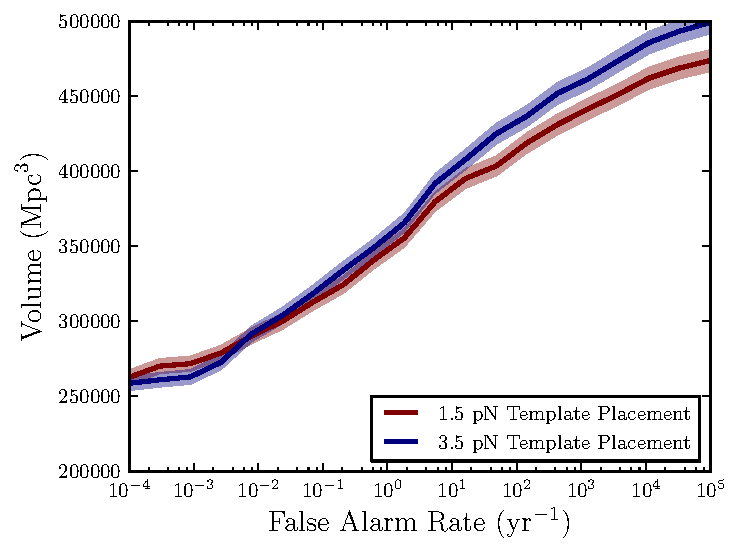
\includegraphics[width=0.45\textwidth]{figures/volume_plots/bank_pn_order_w1_volume.pdf}
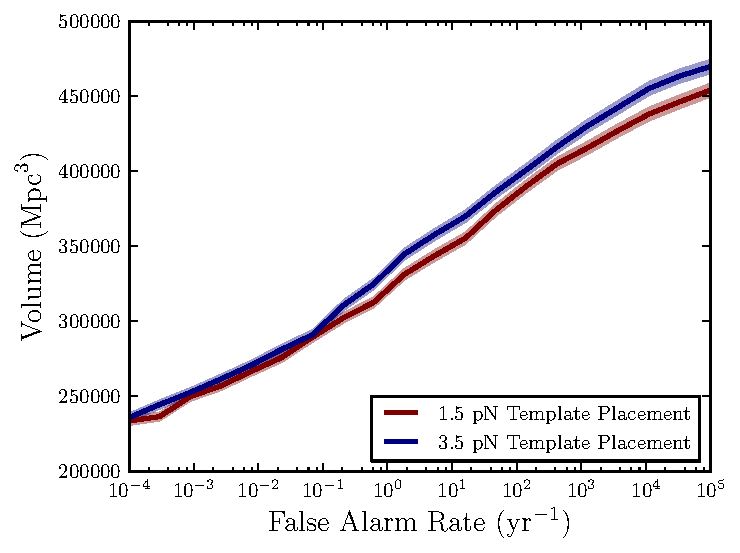
\includegraphics[width=0.45\textwidth]{figures/volume_plots/bank_pn_order_w2_volume.pdf}
\caption{This volume plot compares the analysis with a 3.5 PN bank to our
previous analyses with a 1.5 PN bank week of S6 data. The red line shows that
of the single-stage analysis with a 1.5 PN bank and the blue line shows the
single-stage analysis with a 3.5 PN bank. The left plot represents a week
analysis of data from July 2010 while the right plot represents an analysis of a week of data
from August 2010.} 
\label{img:ahope_15}
\end{center}
\end{figure}


\subsection{Power Spectra Used for Bank Placement}
\label{s:fixed}

Since the shape of the detector's power spectral density changes over time,
the S6/VSR2,3 analysis recomputed the noise power spectral density used in the
matched filter every 2048 seconds. Furthermore, the template banks used in the
search were also regenerated on the same cadence. Since the power spectral
densities of the detectors in the network are not the same, the template bank
was computed independently for both detectors. Since the placement of
templates is not identical between detectors, the pipeline must use a
coincidence test that allows for mismatch between the mass parameters of a
signal. We investigate an alternative method for generating and placing
the template bank. Rather than re-generating the bank every 2048 seconds, we
explore the creation of a single, fixed bank for the entire duration of the
(one week) analysis by averaging the detector's noise power spectral density over the full
analysis time and using this globally averaged power spectral density to place the template bank.

We initially try independently averaging the power spectral density from each detector, creating
separate banks for each detector. We then test the use of a single, fixed bank 
for both detectors by further averaging the power spectral density between the two detectors. 
Using a bank shared between detectors allows us to use a new coincidence testing code,
described in Sec.~\ref{s:coinc} which requries the mass parameters to be
identical in a coincident trigger. To compare the different power spectral
density estimations, we tested several different averaging methods and
compared their relative sensitive volumes. We
begin by considering several methods to average the power spectral density over a week of
gravitational-wave data. The methods used are:
\begin{enumerate}
\item Separate Harmonic Mean.
We first create a single bank for each detector for the duration of the search. 
We measure the power spectral density of the noise every 2048 seconds to 
construct $N$ power spectra $S_n$, as in the existing template placement. We then
construct the harmonic mean power spectral density defined by averaging each
of the separate $f_k$ frequency bins according to
\begin{equation}
S_n^\mathrm{harmonic}(f_k) = N \left/ \sum_{i=1}^N \frac{1}{S_n^i(f_k)} \right.\, .
\end{equation}
The use of the harmonic mean was motivated by Ref.~\cite{Keppel:2013uma} which
shows that the harmonic sum of the individual detector power spectral
densities in a network yields the same combined signal-to-noise ratio as a
coherent analysis of the detector data. The harmonic mean
$S_n^\mathrm{harmonic}(f_k)$ is then used to place a single template bank that
is used for the entire search using one week of data.
Our first test generated an independent harmonic mean power spectral density
for each detector, and so separate template banks were generated for each detectors.
These banks are used for match-filtering in their respective
detectors and the resulting gravitational-wave candidates undergo a
coincidence test between detectors using the ellipsoidal coincidence test.

\item Shared Harmonic Mean.
We next average the power spectral density between the two detectors
to create a single template bank that is shared by both detectors 
(i.e. each detector shares exactly the same templates from a single bank). 
This fixed bank was averaged over the week-long data set
and was used for the entire analysis. After being match-filtered against the
data and the gravitational-wave candidates identified, the ellipsoidal coincidence
test is applied.

\item Shared Smallest-value Estimation.
Our last configuration created a single bank between the two detectors while
choosing the smallest value for the power spectral density. 
The smallest value in each frequency bin represents the best performance of the detector.
The template banks generated by the smallest value power spectral density give
typically a higher number of templates than the other averaging methods.
 Thus by using the smallest value for
each bin of the power spectral density, we can create the most densely packed
bank of templates possible.
\end{enumerate}
Fig.~\ref{different-psds} shows the power spectral density computed for a week of data using
these different averaging methods and the difference of these methods to the
arithmetic mean of the power spectral density.

To test how each of these banks affect the search sensitivity, we performed
several analyses with these different averaging methods.
The results of these investigations are shown in
Fig.~\ref{fig:ave} which compares the sensitive volume as a function of
false-alarm rate. For the first week of data from July 2010, which has large
fluctualtions in the inspiral range, the fixed
template banks have approximately the same sensitivity as the regenerated
template banks for high estimated false alarms rates. For false-alarm rates
of $\sim 10^{-3}$ per year, the bank generated using the fixed harmonic-mean
power spectral density gives the best sensitive volume.
For the second week of data from August 2010, which has a more stable
inspiral range, all of the bank placement methods have the same sensitivity,
within measurement error. In the case when fixed banks provide increased
sensitivity, the harmonic mean gives the best sensitiviy, so we recommend this
averaging method for the search.

We also note that using a fixed template bank reduces the overall
computational cost of the search. Table~\ref{table:cost} shows that the cost
of generating the template banks used here is a small fraction of the overall
run time of the search. Fixing the template bank essentially eliminates this
cost, but since the cost of the bank generation is less than 1\% of the
overall computational cost, this is not a significant saving.  However, for
searches that incorporate compact-object spin in the waveform templates,
template bank generation can be significantly more
expensive~\cite{Harry:2009ea,Brown:2012qf,Canton:2014ena}. For example, for
searches for binary neutron stars between $1$--$3\ M_\odot$  and dimensionless
spins up to $\chi \le 0.4$, or for neutron star--black hole binaries with black
holes masses between $3$ and $15\ M_\odot$ and spins up to $\chi = 1$, the
cost of generating the template bank is three to four orders of magnitude more
expensive than the cost of the bank used here (depending on the low-frequency
sensitivity of the detector). However, the number of templates in the bank, and
hence the cost of matched filtering, only increases by a factor of $2$--$5$.
If the template bank is re-generated every 2048 seconds for 
searches for binaries with spin, bank placement can become a significant fraction of the
overall search cost. The power spectral density averaging methods proposed
here to generate a fixed template bank can be applied to those searches,
significantly reducing the computational cost~\cite{Canton:2014ena}.

\begin{figure}[t!bp]	
\begin{center}
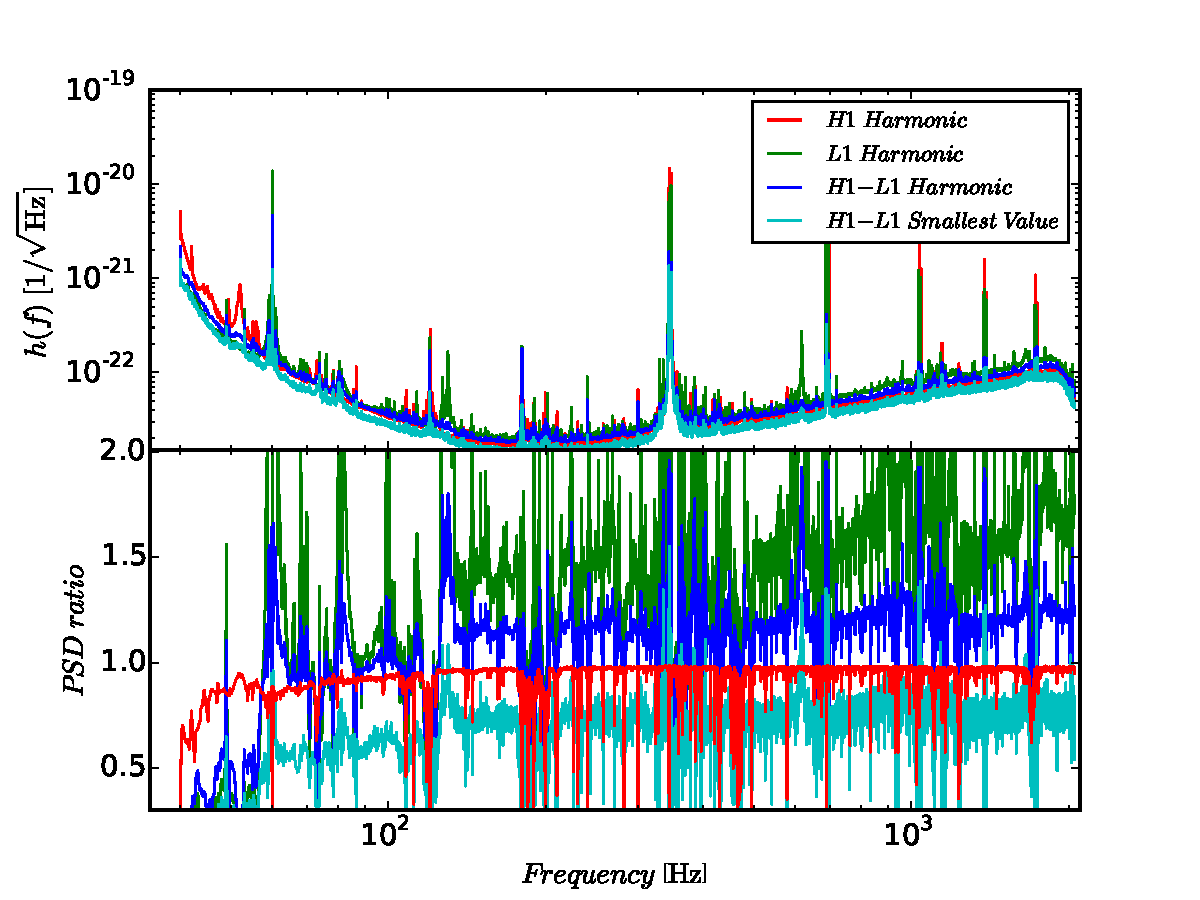
\includegraphics[width=0.65\linewidth]{figures/psd_comparison.pdf}
\caption{The top panel shows the power spectral densities for different
averaging methods of the measured power spectral densities for the one-week
time interval July 08-15, 2010 for the LIGO Livingston (L1) and LIGO Hanford
(H1) detectors.  The lower panel demonstrates the ratio of the
different power spectral densities to the arithmetic mean power spectral
density of the LIGO Hanford Detector.}
\label{different-psds}
\end{center}
\end{figure}

\begin{figure}[t!bp]	
\begin{center}
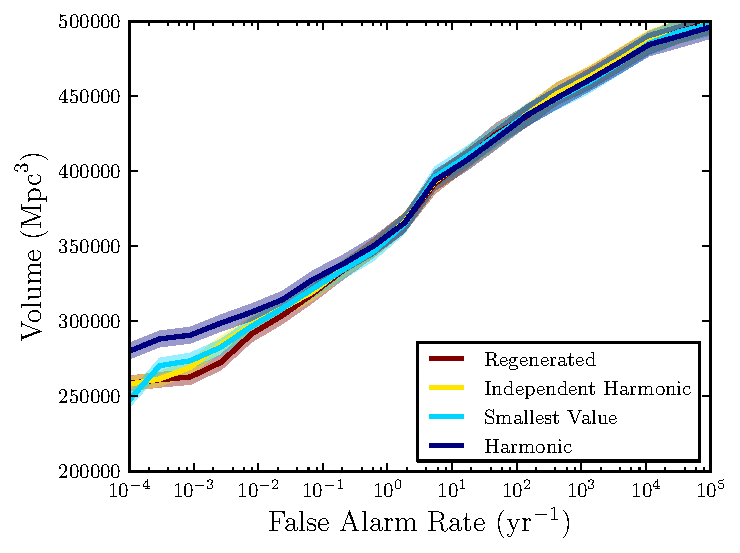
\includegraphics[width=0.45\textwidth]{figures/volume_plots/compare_psd_average_w1_volume.pdf}
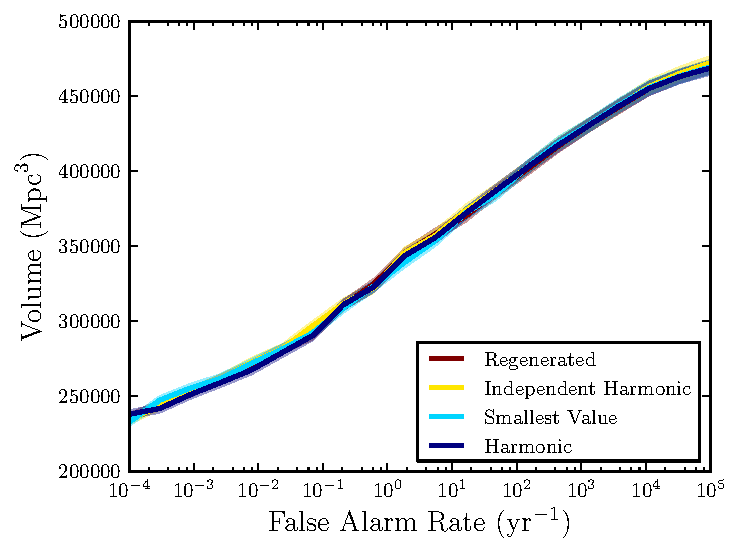
\includegraphics[width=0.45\textwidth]{figures/volume_plots/compare_psd_average_w2_volume.pdf}
\caption{This volume plot describes the sensitive volumes of the searches in
different configurations. The red line is an analysis using template banks
regenerated every 2048 s. The blue, yellow and cyan lines show different
analyses with fixed banks. The blue and yellow used a harmonic mean to
estimate the power spectral density, while the cyan simply chose the lowest power spectral density measured at each
frequency. The regenerated-bank and the independent-harmonic analyses used
separate banks for the different detectors, while the smallest-value and
harmonic analyses used a common bank for both detectors. The left plot
represents an analysis of a week of data from July 2010 while the right plot represents a week
analysis of data from August 2010.}
\label{fig:ave}
\end{center}
\end{figure}

\subsection{Trigger Coincidence Test}
\label{s:coinc}

Since the S6/VSR2,3 search used separate regenerated template banks for each
detector, a coincidence test that allows triggers to have slightly different
mass parameters must be used in the search. The template placement metric was
used to construct the ellipsoidal coincidence test which determines if two
waveforms are coincident in time and mass between
detectors~\cite{Robinson:2008un}. Tuning the size of the ellipsoidal
coincidence test is performed empirically by calculating the distribution of
the ellipsoidal coincidence window for simulated signals and for noise events
from the background time shifts, and choosing a value of the parameter
controlling the size of the ellipse that provides the best separation of
signals and background. 

Using a shared, fixed bank for both detectors allows us to investigate a
new, simpler type of coincidence test. In this \emph{exact-match} coincidence
test, we use the ellipsoidal window to determine if triggers are coincident in
time, since there is still a time-of-flight difference between triggers in the
detectors, however we require that the mass parameters $m_1$ and $m_2$ of the
template are exactly the same in both detectors. 
This requirement
decreases the chance that triggers generated by noise
transients will be found in coincidence between detectors, as it is a stricter
test than the ellipsoidal test.
The exact-match method of testing for coincidence
is useful in situations where there is no simple metric to compare
gravitational waveforms, as is the case with template waveforms for binaries
with spinning neutron stars or black holes\cite{Canton:2014ena}.

In Fig.~\ref{fig:coinc}, we compare the performance of the search on two weeks
of S6 data using the same, fixed harmonic bank in both detectors, but using
either the ellipsoidal coincidence test or the exact-match coincidence test.
The ellipsoidal coincidence test tends to recover injections with higher
combined reweighted signal-to-noise ratio than exact-match test: the less
stringent ellipsoidal coincidence test allows more templates in each detector
to contribute to coincidence, thus there is more chance of an upwards
fluctuation in the detection statistic.  The gain in sensitivity from the
exact-match test is a tradeoff between the (on average) smaller
signal-to-noise ratio of signals and the lower background level, giving an
increase in detection significance at a given signal-to-noise ratio.  For the
week from July 2010, the performance of the exact-match coincidence test is
slightly better than that of the ellipsoidal test, although the difference is
within the error bars at a false-alarm rate of $10^{-3}$ per year.  However,
for the week from August 2010, the sensitivity of the search using the 
exact-match test is clearly higher at a false-alarm rate of $10^{-3}$ per year. 

We can understand this increase using Figs.~\ref{fig:ethinca_hist} and 
\ref{fig:exact_hist},
which compare histograms of the combined reweighted signal-to-noise ratio of
background triggers obtained in S6 data to Gaussian noise. For the first week of
data, the distribution of background triggers using the ellipsoidal
coincidence test, shown in Fig.~\ref{fig:ethinca_hist}, is very close to that
of Gaussian noise. However, for the second week, the S6 data contain more
triggers at higher combined reweighted signal-to-noise ratio. This difference
can still be seen in Fig.~\ref{fig:exact_hist}, which shows the distribution
of background triggers from the exact-match coincidence test.  Note, also, 
that in the exact-match analysis, the overall rate of triggers is significantly
lower for both weeks, resulting in lower false-alarm rate at a given value of 
combined reweighted signal-to-noise ratio.  Our results show that the lowering
of the noise background with exact-match coincidence is the dominant effect: 
signals are recovered with greater significance, raising the search sensitivity.
 
\begin{figure}[t!bp]	
\begin{center}
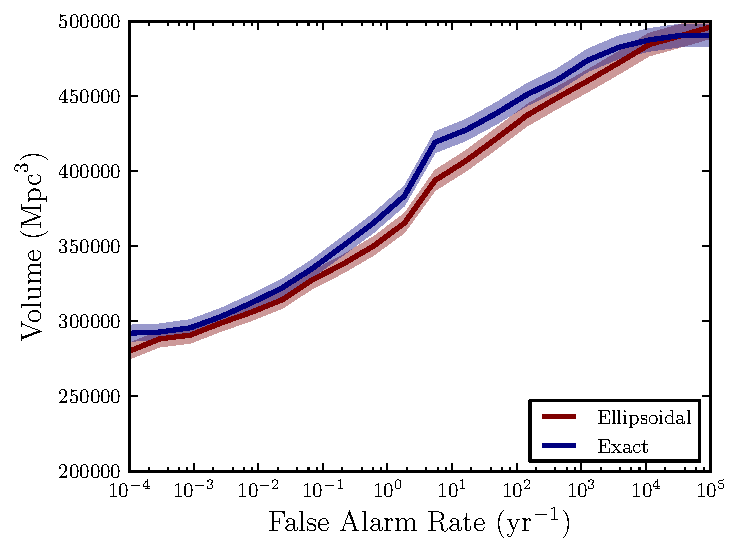
\includegraphics[width=0.45\linewidth]{figures/volume_plots/ethinca_exact_match_w1.pdf}
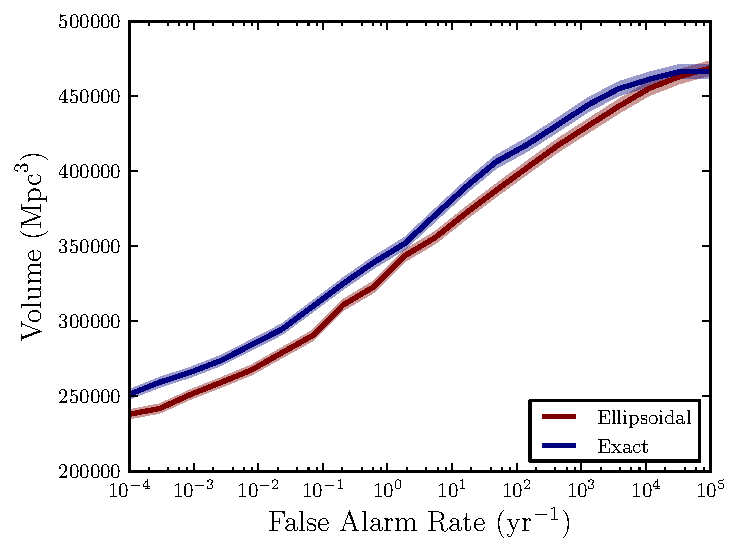
\includegraphics[width=0.45\linewidth]{figures/volume_plots/ethinca_exact_match_w2.pdf}
\caption{This volume plot describes the relative sensitive volumes of the
different search pipelines as a function of false-alarm rate. The red curve
describes the sensitivity of a search pipeline using the ellipsoidal coincidence test.  
The blue curve
demonstrates the sensitivity of the search pipeline using a fixed bank and the
new exact-match coincidence test. The left plot represents a week
analysis of data from July 2010 while the right plot represents an analysis of a week of data
from August 2010.}
\label{fig:coinc}
\end{center}
\end{figure}

\begin{figure}[tbp]
\begin{center}
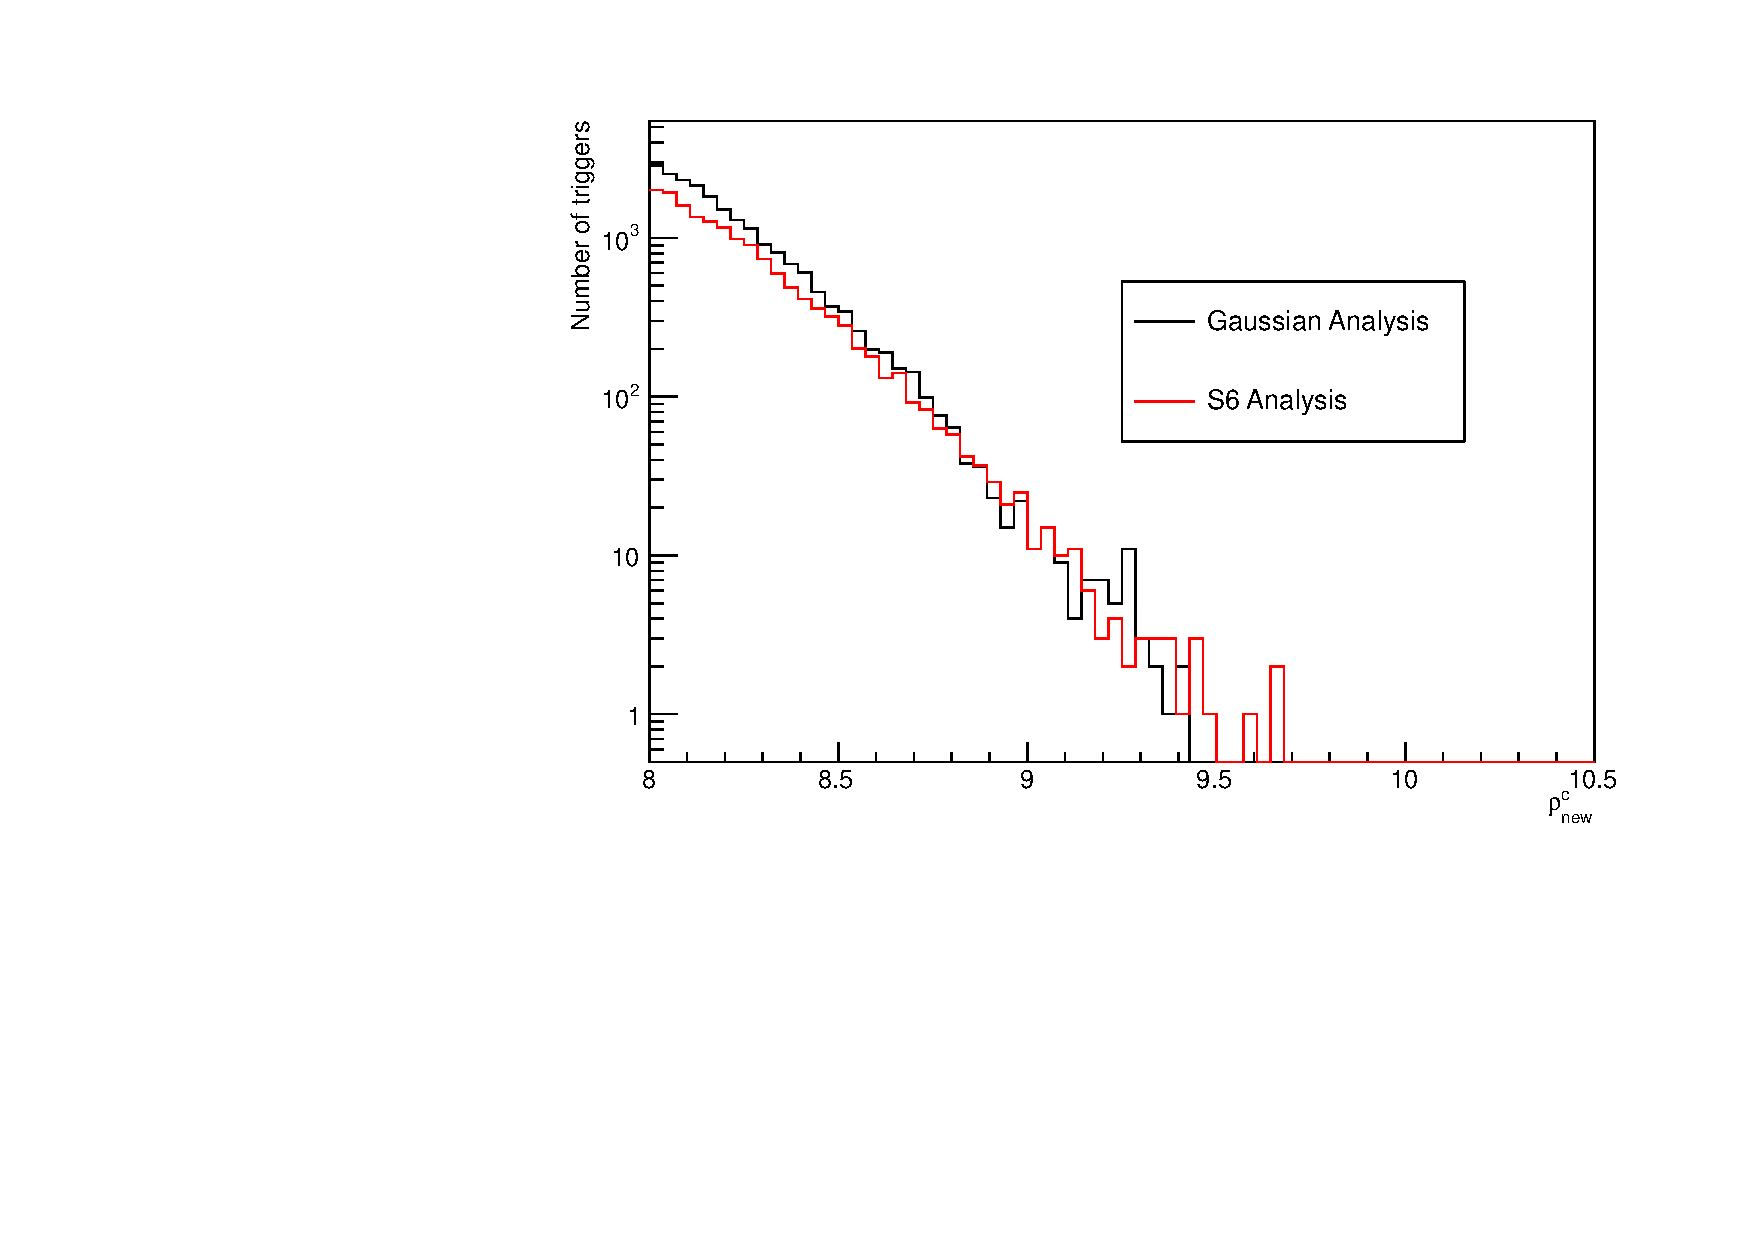
\includegraphics[width=0.45\textwidth]{figures/histograms/same_harm_ethinca_gaussian_vs_s6_w1.pdf}
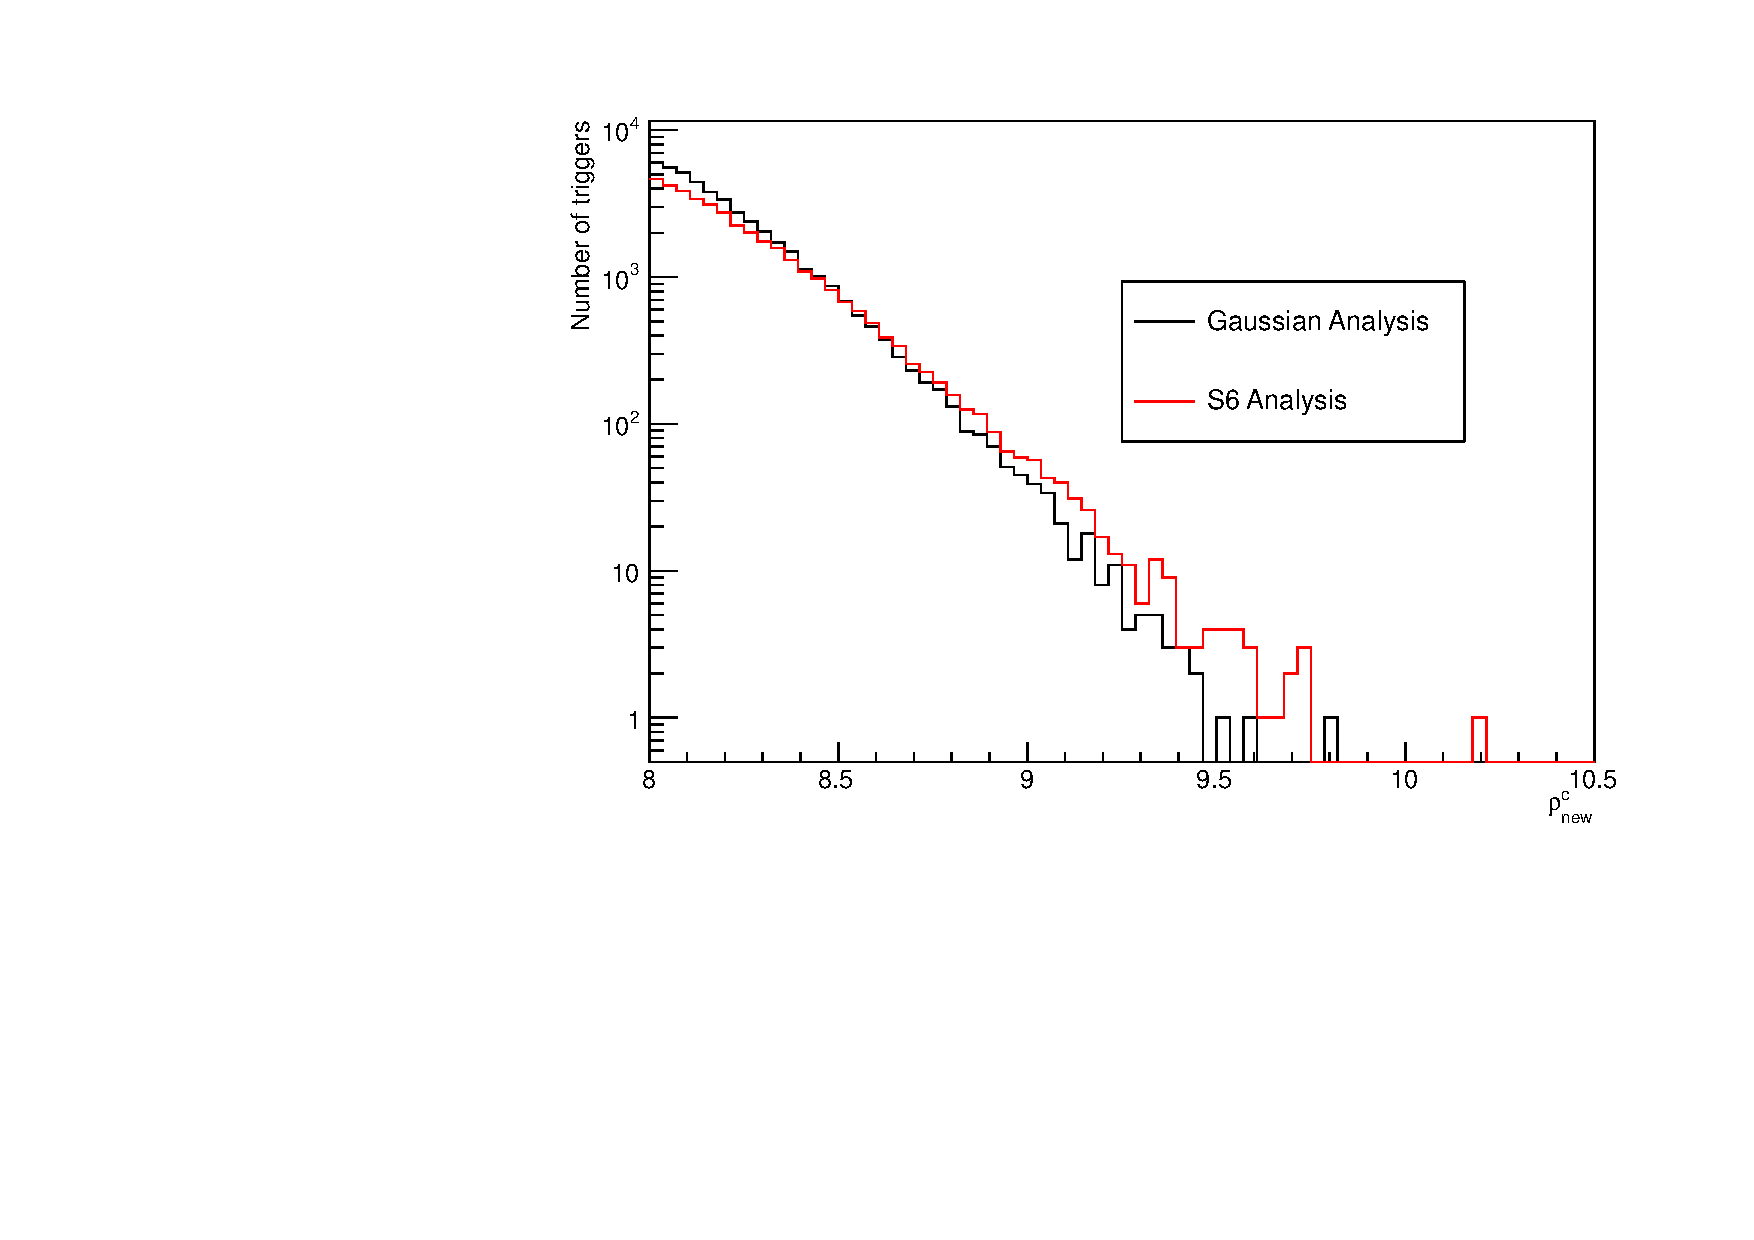
\includegraphics[width=0.45\textwidth]{figures/histograms/same_harm_ethinca_gaussian_vs_s6_w2.pdf}
\caption{This histogram shows the number of background triggers that survived
coincidence testing from the analysis using a shared, fixed harmonic bank using
ellipsoidal coincidence testing in different bins of combined reweighted signal-to-noise ratio.
The red line denotes the background triggers from the Gaussian analysis.  The
black line denotes the background triggers from the S6 data analysis. The left
plot represents an analysis of a week of data from July 2010 while the right plot represents a
week analysis of data from August 2010.}
\label{fig:ethinca_hist}
\end{center}
\end{figure}

\begin{figure}[tbp]
\begin{center}
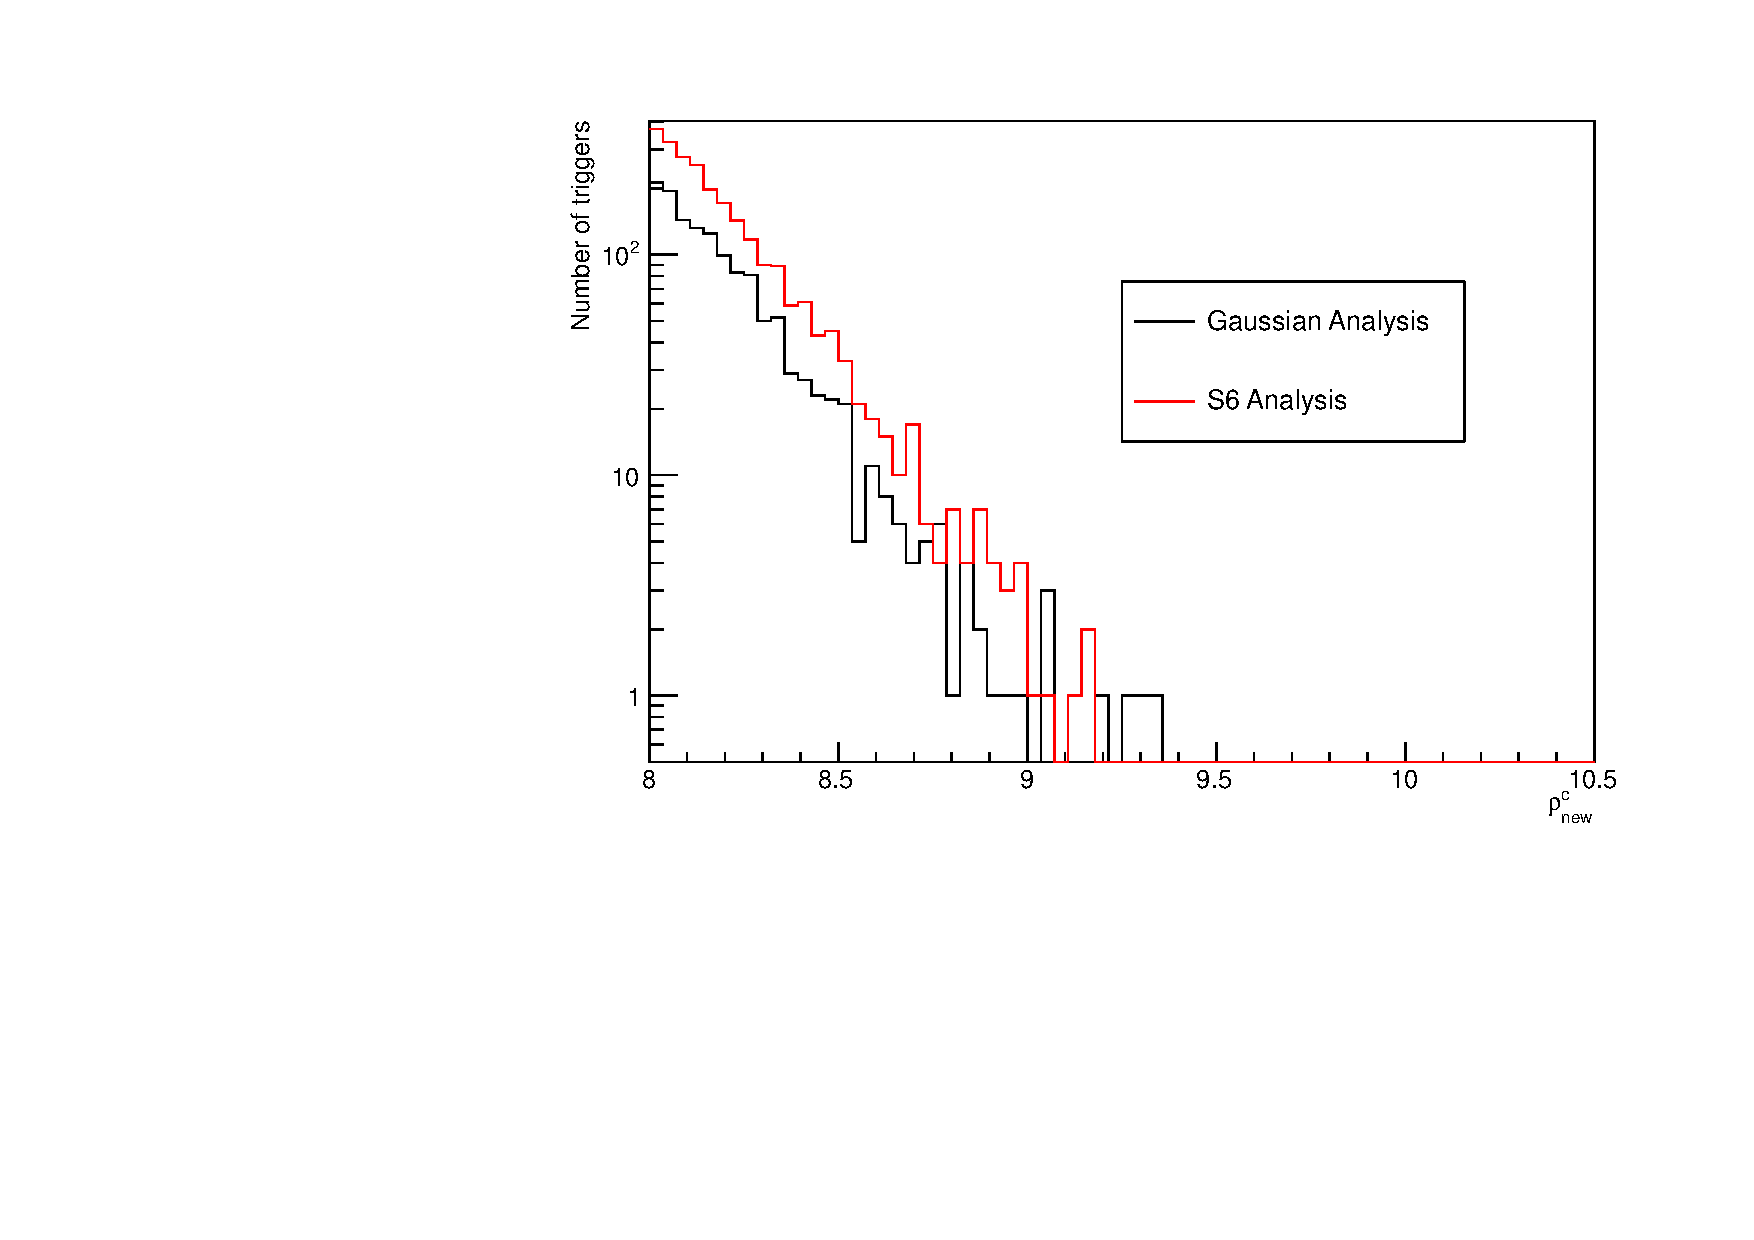
\includegraphics[width=0.45\textwidth]{figures/histograms/same_harm_exact-match_gaussian_vs_s6_w1.pdf}
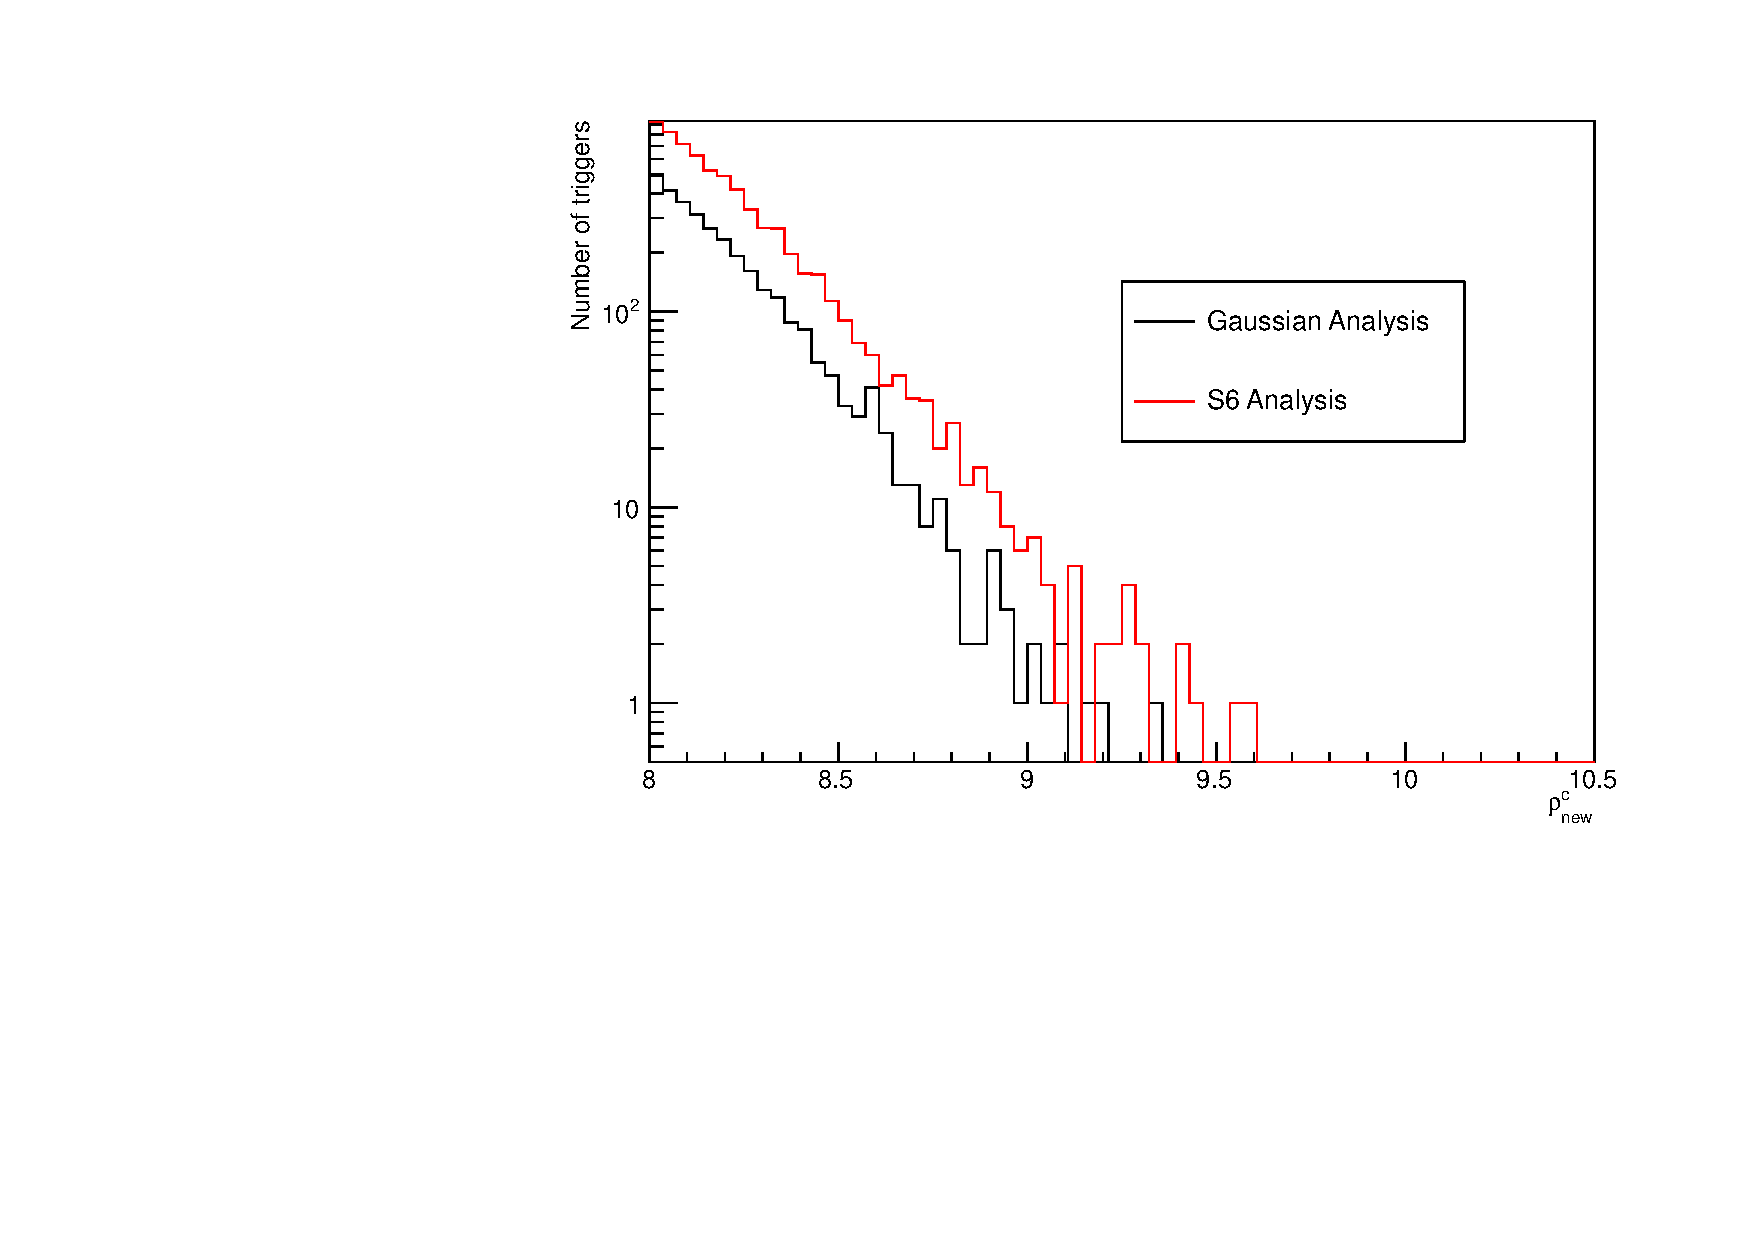
\includegraphics[width=0.45\textwidth]{figures/histograms/same_harm_exact-match_gaussian_vs_s6_w2.pdf}
\caption{This histogram shows the number of background triggers that survived
coincidence testing from the analysis using a shared, fixed harmonic bank
using \texttt{exact-match} coincidence testing in different bins of combined
reweighted signal-to-noise ratio. The red line denotes the background triggers from the Gaussian
analysis.  The black line denotes the background triggers from the S6 data
analysis. The left plot represents an analysis of a week of data from July 2010
while the right plot represents an analysis of a week of data from August 2010.}
\label{fig:exact_hist}
\end{center}
\end{figure}
 
\begin{figure}[t!bp]	
\begin{center}
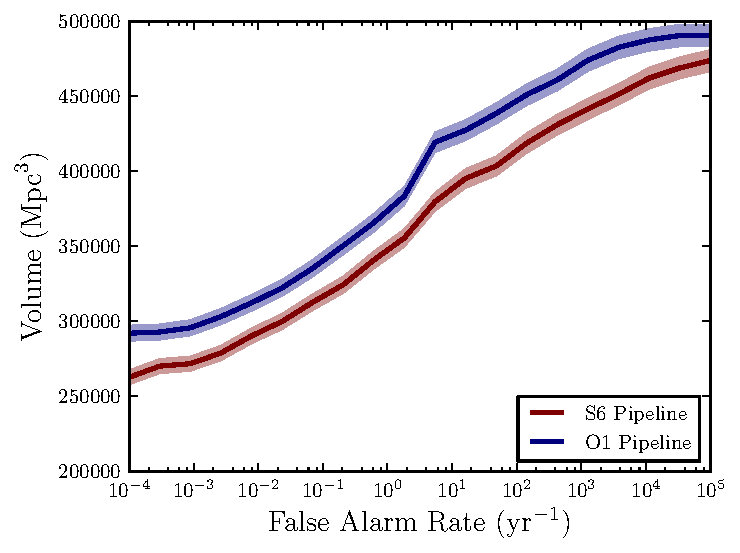
\includegraphics[width=0.45\linewidth]{figures/volume_plots/final_configuration_w1.pdf}
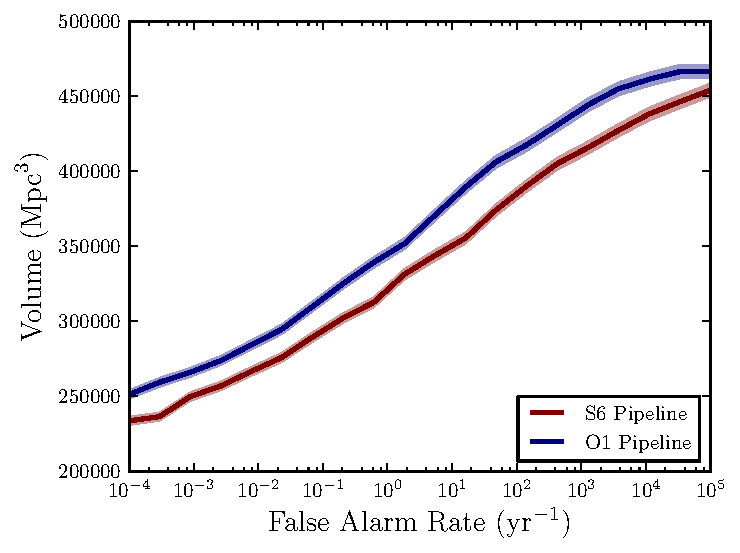
\includegraphics[width=0.45\linewidth]{figures/volume_plots/final_configuration_w2.pdf}
\caption{This volume plot describes the relative sensitive volumes of the
different search pipelines as a function of false-alarm rate. The red curve
describes the sensitivity of the search pipeline used in LIGO's sixth science
run, reformatted to have a single coincidence test.  The blue curve
demonstrates the sensitivity of the search pipeline using a fixed bank and the
new exact-match coincidence test. The left plot represents an
analysis of a week of data from July 2010 while the right plot represents an
analysis of a week of data from August 2010.}
\label{fig:conc}
\end{center}
\end{figure}

\section{Conclusion}
\label{s:conc}

We have demonstrated the use of a new pipeline to search for gravitational
waves from compact object binaries in LIGO data.  The results of our study are
summarized in Fig.~\ref{fig:conc} which compares the sensitivity of the search
pipeline used in S6/VSR2,3 (analysis 1 of Table~\ref{table:search}) with the
most sensitive pipeline proposed here (analysis 8 of Table~\ref{table:search})
which uses a shared fixed 3.5pN template bank in both detectors generated using 
a harmonic mean power spectral density, and the exact-match coincidence test.  
We see that these improvements result in a gain of $\sim 10\%$ in the sensitive
volume of the search at a false-alarm rate of $10^{-3}$ per year. %We can see
%from the above analysis that this gain comes from different modifications to
%the pipeline, depending on the quality of the LIGO data. For the first week of
%data from July 2010, the improvement mainly comes from using the fixed
%template bank for the week of analysis. For the second week, the improvement
%mainly comes from the use of the exact-match coincidence test.
The new pipeline uses a simpler, single-stage workflow that allows us to
estimate false-alarm rates to $\sim 10^{-4}$ per year using one week of data. With our improved
implementation of the $\chi^2$ signal-based veto, we demonstrate that the new
pipeline has the same computational cost as the two-stage workflow used in the S6/VSR2,3
analysis. We propose that this workflow be used as a basis for offline
searches for gravitational waves from compact-object binary sources in aLIGO
and AdV.

We note that a new class of search pipeline was prototyped in
S6/VSR2,3~\cite{Abbott:2011ys} that produces triggers in low-latency for rapid
follow-up by electromagnetic observatories. These pipelines are under
active development for aLIGO and AdV~\cite{Adams:MBTA,Cannon:2011vi}.
Low-latency searches differ from the pipeline presented here as they are constrained to
only use information available in the past and trade computational cost for
speed of producing detection candidates. However, since they are 
based on coincident matched filtering, our results can also be
used to inform the development of low-latency searches. For example, we would expect
that the harmonic mean (using recent past detector data) would provide the best
power spectral density estimation for the construction of template banks used
in the singular value decomposition proposed in Ref.~\cite{Cannon:2011vi}.
Similarly, we expect that exact-match coincidence would provide the best
coincidence method for the low-latency pipelines.

Finally, we note that Figs.~\ref{fig:ethinca_hist} and \ref{fig:exact_hist}
show that, although the distribution of triggers in the S6 search using the
ellipsoidal test is very close to that of Gaussian noise this is not the case
for exact-match. This suggests that additional tuning is possible to increase
the sensitivity of the search. Investigation of improved tuning could explore
the optimal length of time for a single bank, further tuning of the
coincidence test, improvements to power spectral density estimation used in
the matched filter, improved signal-based vetoes and optimization of the
combined detection statistic. Further tuning beyond what is presented here
will be the subject of future studies. 

\ack
CMB, DAB, AHN, and SAU acknowledge support from NSF awards PHY-0847611 and
PHY-1404395 and a Research Corporation for Science Advancement Cottrell
Scholar Award. IWH, PRS and MW acknowledge support from NSF awards PHY-0854812 and
PHY-1205835. MSK, IWH, CDC, TD, TDC, JLW, and DK acknowledge
and thank the support of the Max-Planck-Gesellschaft. 
MSK is also greatful for
hospitatility of the Max-Planck-Institut f{\"u}r Gravitationsphysik in Golm where part
of this work was carried out.
Computations used in this analysis were performed on the
Syracuse University SUGAR cluster, supported by NSF awards PHY-1040231 and
PHY-1104371, and by Syracuse University ITS, as well as the ATLAS cluster
supported by the Max-Planck-Gesellschaft.

%=============================================================================
\section*{References}
%\bibliographystyle{unsrt-notitle}
\bibliographystyle{iopart-num.bst}
\bibliography{cbc_ahope_paper}

\end{document}
